\documentclass[10pt,twocolumn,letterpaper]{article}

\usepackage{cvpr}
\usepackage{times}
\usepackage{epsfig}
\usepackage{graphicx}
\usepackage{amsmath}
\usepackage{amssymb}
\usepackage{subfigure}
\usepackage{algorithmic}
\usepackage{algorithm}

\newenvironment{tightenumerate}{
\begin{enumerate}
  \setlength{\itemsep}{1pt}
  \setlength{\parskip}{0pt}
  \setlength{\parsep}{0pt}
}{\end{enumerate}
}

% this makes list spacing much better.
\newenvironment{tightitemize}{
\begin{itemize}
  \setlength{\itemsep}{1pt}
  \setlength{\parskip}{0pt}
  \setlength{\parsep}{0pt}
}{\end{itemize}
}

\cvprfinalcopy % *** Uncomment this line for the final submission

\def\cvprPaperID{****} % *** Enter the CVPR Paper ID here
\def\httilde{\mbox{\tt\raisebox{-.5ex}{\symbol{126}}}}

% Pages are numbered in submission mode, and unnumbered in camera-ready
\ifcvprfinal\pagestyle{empty}\fi

\begin{document}

\title{Attributes-based Object Classification and Segmentation}

\author{Aibo Tian and John Edwards\\
University of Texas at Austin\\
%Institution1\\
%Institution1 address\\
{\tt\small \{atian,edwardsj\}@cs.utexas.edu}
% For a paper whose authors are all at the same institution,
% omit the following lines up until the closing ``}''.
% Additional authors and addresses can be added with ``\and'',
% just like the second author.
% To save space, use either the email address or home page, not both
%\and
%John Edwards\\
%Institution2\\
%First line of institution2 address\\
%{\tt\small edwardsj@cs.utexas.edu}
%University of Texas at Austin\\
}
%University of Texas at Austin\\

\maketitle
\thispagestyle{empty}

%-------------------------------------------------------------------------------
% abstract
%-------------------------------------------------------------------------------
\begin{abstract}
Attributes have been shown to be effective in assisting object classification and
classification, and they provide means to also incorporate semantic
information available to and provided by humans.  On another front, the
combination of segmentation and object classification has been shown to
improve both segmentation and classification.  We present a method of incorporating
attributes into segmentation using a hierarchical methodology.
That is, using attributes as features, we discover attributes of regions
at all levels of a hierarchical segmentation,
incorporate hierarchical confidences in determining a confidence that
a given region is part of a given object, and segment the image using
these confidences.  We also present encouraging segmentation results
from experiments run using this method.
\end{abstract}

%-------------------------------------------------------------------------------
% introduction
%-------------------------------------------------------------------------------
\section{Introduction}
Very recent work on using attributes as features \cite{farhadi09, lampert09}
has shown that attributes are an effective way of communicating information
about an object in an image.  Attributes are, in essence, semantic high-level
features.  The attributes of an image are learned using low-level features,
and once learned, they can be used in object classification and also in describing
objects in an image that are unknown.

Image segmentation is a very different field of research and has a very different
goal - that of finding very accurate boundaries of objects in an image.

Our work focuses on leveraging attributes to produce accurate segmentations.
The idea is to find image regions with attribute distributions very similar
to some canonical distribution for an object.  Figure \ref{fig:truck} shows
an example.  We define the ``canonical distribution''
to be an attribute distribution representative of that object.  For example, the
canonical distribution for a ``car'' would have some measure of ``shininess'', some
other measure of ``window'' and so forth.  If
regions can be combined together to for larger regions with attribute
distributions matching the object's canonical distribution then one can
declare the combined region an accurate segmentation for that object.

%We note that it is possible that one segmented region may contain the object and
%nothing else.  Though possible, in practice it is highly unlikely.  Even for rather
%simple objects, the true region of the object is distributed among various
%segmentations.  This is because all but the most trivial objects have different
%sub-regions of different colors, textures, contours, etc.  Thus we must search
%for a combination of these sub-regions that make up the object.


\begin{figure}
\centering
\subfigure[]{
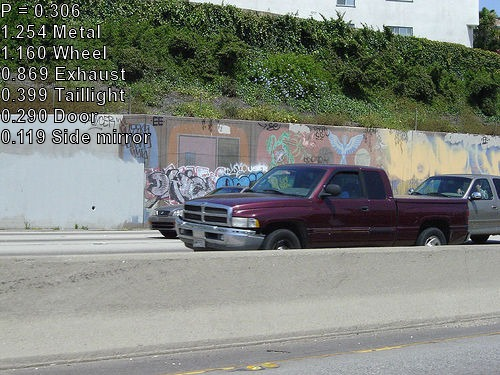
\includegraphics[width=0.22\textwidth]{figures/truck_orig_med.eps}
\label{fig:trucka}
}
\subfigure[]{
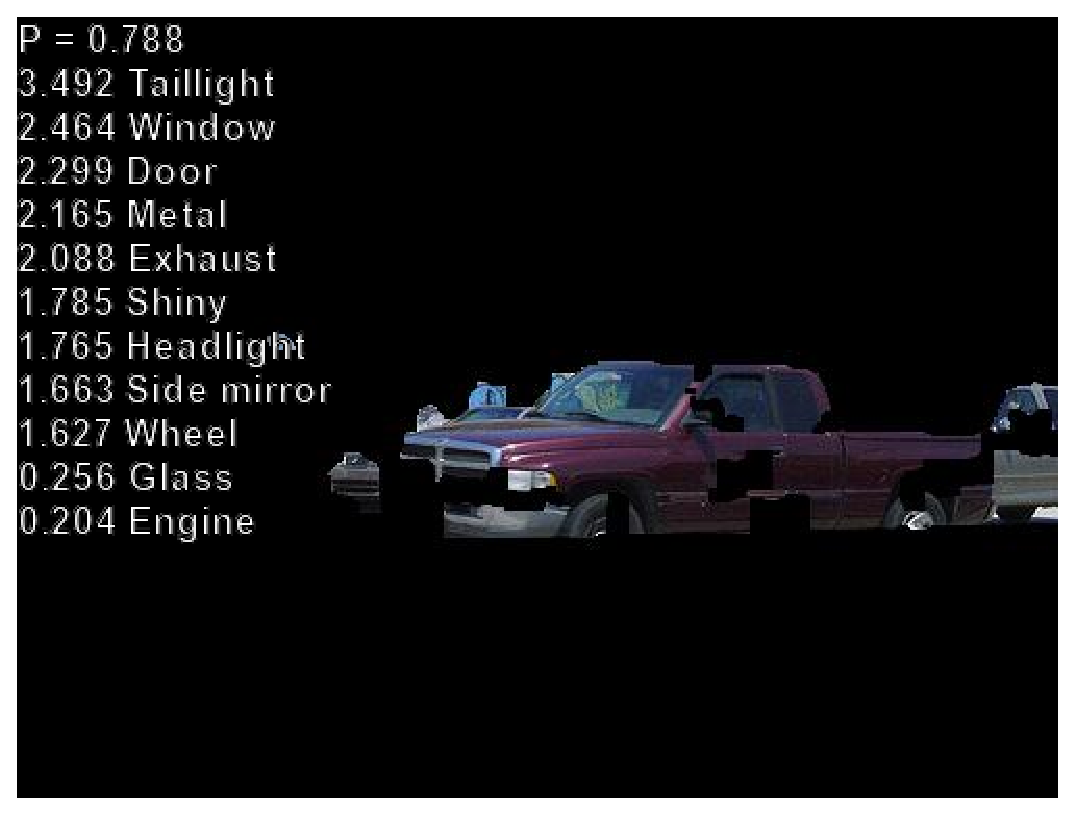
\includegraphics[width=0.22\textwidth]{figures/truck_final_med.eps}
\label{fig:truckb}
}
\caption{Segmentation by maximizing attribute similarity to a canonical
attribute distribution for a car.  \subref{fig:trucka} shows
the original image with any ``car'' attributes that were predicted.  $P$ is the probability
that the image contains a car.  \subref{fig:truckb} shows the segmented image after
running our segmentation tree pruning algorithm.  As extraneous regions are pruned
more car attributes are predicted and the probability that the remaining image
contains a car increases.}
\label{fig:truck}
\end{figure}

In general, the testing of all combinations of regions to
find objects is intractable.  We use two approximatory algorithms
operating on a segmentation hierarchy to determine regions belonging
to a given class.
One algorithm is additive and operates by combining regions that are likely
to be part of the object.  The other is subtractive, which first predict attributes on
the entire region and then proceeds by observing the effects of
removing different regions during a top-down traversal of the tree.
The benefit of using these methods are that large regions that
clearly don't contribute to an attribute distribution similar to the
canonical can be pruned from
the tree early in the traversal.  This approach avoids the
combinatoric complexity of a full search and, even more, prunes many
regions from the segmentation tree before they even are searched,
bringing the computational complexity, in practice, to roughly
$O(n)$ where $n$ is the number of leaves in the segmentation tree.
The flowchart of our algorithm is shown in Figure
\ref{fig:flowchart}.

This work is done using attributes as the features, but the segmentation
pruning algorithms are actually feature-type agnostic and could be used
with any image feature given a scoring function applicable to that feature.

While we focus on segmentation of known objects, we anticipate an application
that takes more advantage of attributes: that of segmenting \emph{unknown}
objects from an image that exhibit stable but unrecognized attribute
distributions.  This type of application brings out some of the true power of
attributes, that of assigning semantic meaning to unknown, segmented objects.

%This paper is organized as follows: we first discuss related work (\S \ref{sec:related_work})
%and then present the algorithm in detail (\S \ref{sec:technical}).  We then discuss results from
%a small-scale experiment on images from the pascal 2008 dataset (\S \ref{sec:results}), after which we draw
%conclusions and discuss future directions (\S \ref{sec:conclusions}).

%-------------------------------------------------------------------------------
% related work
%-------------------------------------------------------------------------------
\section{Related work}
\label{sec:related_work}

\begin{figure}
\centering
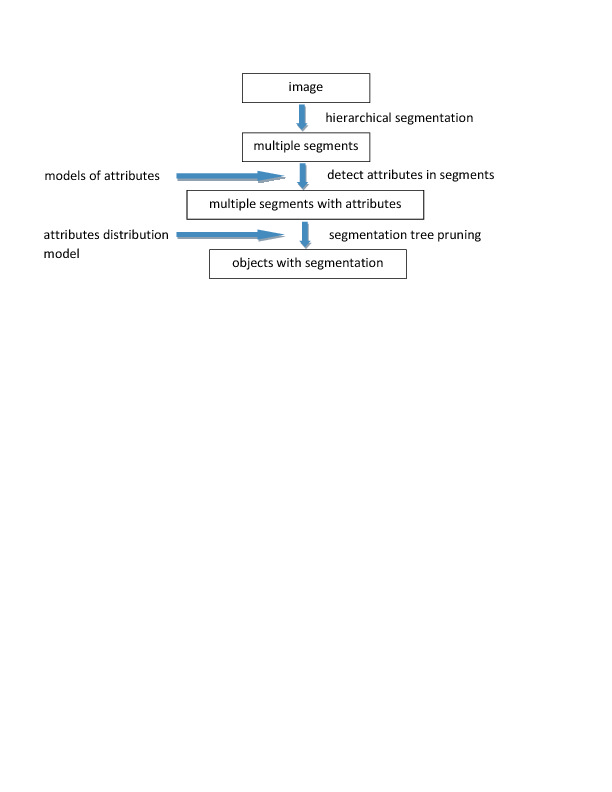
\includegraphics[width=0.5\textwidth]{figures/flowchart.eps}
\caption{Flowchart of the proposed algorithm.} \label{fig:flowchart}
\end{figure}

A significant amount of recent work has been done in the area of using
attributes as high-level features for image classification and object
description \cite{farhadi09, lampert09, kumar09}.
Another area of computer vision, that of segmentation,
has seen a resurgence of popularity as methods to incorporate top-down
information into segmentation have been shown to be highly effective
\cite{borenstein04, pantofaru, gu09, russell06, malisiewicz, leibe04, hoiem05, shotton06}.
We propose to leverage research done in both of these areas -- attributes
and top-down/bottom-up segmentation -- to produce a combined approach.

Farhadi et al
\cite{farhadi09} use attributes as high-level features for object classification. They
can also describe an image using its attributes alone.
Lampert et al \cite{lampert09}
use the attributes as a intermediate layer between the low-level
features and object classes. Based on this layer, they can predict
disjoint classes that are not seen in the training set.  Both of these
approaches are geared toward object detection and classification.  While
our method goes further, incorporating segmentation, we will be using
the ideas and algorithms in \cite{farhadi09} for assignments of
attributes to different segmented regions.

Object classification can give some top-down high-level information
for segmentation. On the other hand, segmentation can provide
image-based coherence information for classification. To deal with
the problem that the bottom-up single segmentation is not accurate,
more and more algorithms are based on multiple segmentations. Gu et
al \cite{gu09} uses the hierarchical segmentation algorithm to
generate multiple segments, and detect different parts of objects in
each segment. The final objects are voted for by the various parts.
We will initially be using the same segmentation algorithm used in
this paper, but without discarding the hierarchy.

Russell et al \cite{russell06} attempt object classification 
by assuming that most objects get segmented
correctly at least once during the multiple segmentation. We make no such
assumption.  Rather, we find some region that contains the entire
object (which may be the original image) and refine that rough
segmentation.  Russell et all also learn object classes in an
unsupervised manner.  Our approach
will be far less aggressive in that we will use object classes 
that are known \emph{a priori}.
Pantofaru et
al \cite{pantofaru} use three different segmentation algorithms to
generate the multiple segments. After detecting objects in each
segment, they merge the intersected segments as final results. In
our method, we use common knowledge of distribution of attributes to
merge segments.
Borenstein et al \cite{borenstein04} proposed a method of combining top-down
and bottom-up information to generate a high-quality segmentation.  Their
approach to the top-down is to use exemplar image fragments and match them
to the image and then refining the top-down segmentation using their
segmentation hierarchy.  Our approach doesn't use any confidence boosting based
on the hierarchy like they do, but rather, the hierarchy is used to guide
efficient removal and combination of regions.

%Another interesting work is that of Gould et al \cite{gould08}.  They use
%superpixels for an initial segmentation, build a CRF that includes a
%relative location feature in the energy function and minimizes the CRF
%for a final segmentation.  The relative location feature is determined
%using prior location probability maps.  Our approach is similar to this
%as well, in that we will also incorporate relative location information,
%although ours will use attributes' relative locations rather than object
%classes.  We will also use a CRF for the final segmentation, but will
%use a min-cut solution since our labels are binary.
%Kumar et al \cite{kumar05} incorporate shape structure into the segmentation by
%adding a latent shape parameter to the CRF.  This seems like it would be
%a useful addition to our system but make the scope too large.

%\begin{figure}
%\centering
%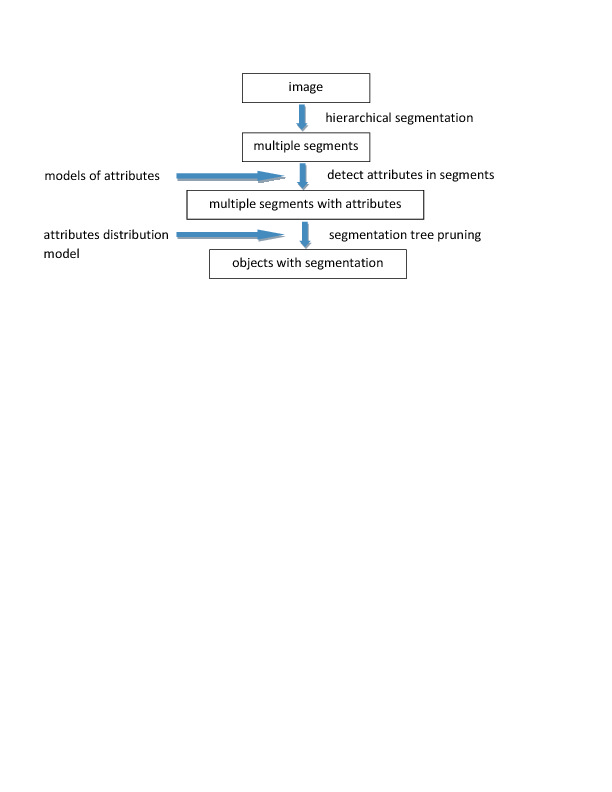
\includegraphics[width=0.5\textwidth]{figures/flowchart.eps}
%\caption{Flowchart of the proposed algorithm.} \label{fig:flowchart}
%\end{figure}


%-------------------------------------------------------------------------------
% technical approach
%-------------------------------------------------------------------------------
\section{Attribute Detection}
\label{sec:attribute}

Attributes are high-level features which can reflect semantic properties of objects. Given the attributes, we can do object detection based on their distribution. We use the same attribute set as \cite{farhadi09}. This set contains three types of attributes, including shape, part and material. All attributes are listed in figure \ref{fig:atts}.

\begin{figure}
\begin{tabular}{llll}
2D Boxy & 3D Boxy & Round & Vert Cyl \\
Horiz Cyl & Occluded & Tail & Beak \\
Head & Ear & Snout & Nose \\
Mouth & Hair & Face & Eye \\
Torso & Hand & Arm & Leg \\
Foot/Shoe & Wing & Propeller & Jet engine \\
Window & Row Wind & Wheel & Door \\
Headlight & Taillight & Side mirror & Exhaust \\
Pedal & Handlebars & Engine & Sail \\
Mast & Text & Label & Furn. Leg \\
Furn. Back & Furn. Seat & Furn. Arm & Horn \\
Rein & Saddle & Leaf & Flower \\
Stem/Trunk & Pot & Screen & Skin \\
Metal & Plastic & Wood & Cloth \\
Furry & Glass & Feather & Wool \\
Clear & Shiny & Vegetation & Leather \\
\end{tabular}
\caption{List of attributes trained.}
\label{fig:atts}
\end{figure}

We use a similar algorithm to that used in \cite{farhadi09} to train the attribute models. 
Three different type of features are used: HOG, texture and color descriptors \cite{farhadi09}.  
We use kmeans to quantize the features. The HOG descriptors are quantized into 1000 clusters, 
and the texture and color are quantized to 256 and 128 clusters, respectively. 
All quantized features are concatenated to form a 1384 dimensional feature.
Since all features are local, we represent a segment by using only features inside the segment
to produce a feature histogram.  In other words, rather than segmenting the image and finding features,
we find features and then segment the features.
This is done to avoid introducing any feature artifacts as a result of black space surrounding 
segmented regions in the image.

For training, we use an SVM classifier with a Gaussian kernel to train
the model for each attribute.  

%The precision of all the attributes on the test set is illustrated
%in figure?.


%Our approach begins with training attribute classifiers.  We trained using
%an SVM with linear kernel.  A set of training images is annotated with objects
%contained in the image, bounding boxes for the objects, and attributes exhibited
%by the image.  We use a subset of the features used in \cite{farhadi09}, namely
%HOG, texture and color descriptors.  The HOG descriptors are quantized into 1000
%kmeans centers, and the texture and color are quantized to 256 and 128 kmeans centers,
%respectively.  Our features differ from \cite{farhadi09} in various ways.  We don't
%use edge descriptors, nor do we generate ``sub-''histograms for 6 cells in the
%image.  The presence of cell histograms would complicate matters when extracting
%features from segmented regions.

\section{Hierarchy Segmentation}
\label{sec:segmentation}

We use the segmentation approach of \cite{arbelaez09}.  This
produces a hierarchical segmentation by first detecting contours
using the \emph{gPb} detector \cite{maire08}.  This contour detector
is advantageous because it uses brightness, color and texture
gradients at multiple scales.  Once the contours are
detected, regions are discovered using a watershed algorithm after
which an Ultrametric Contour Map (UCM) is constructed, which defines
the region hierarchy.  The UCM is stored as a grayscale image with
contours around the segmented regions.  These contours have intensities
representative of the region's location in the hierarchy.  So to find
the first branch in the tree, threshold the UCM image with a value
$t$ where $t = max{I(x,y)}$ where $I(x,y)$ is the intensity at pixel
location $(x,y)$.  The thresholded image can then be flood-filled into
regions.  These regions correspond to the branches on either side of
the root node in the segmentation tree.  The next level of the tree is
found by thresholding the two new regions of the UCM at each, respective,
next highest intensity and so on.
Figure \ref{fig:ucm} shows an example UCM image and figure \ref{fig:tree}
shows the hierarchy generated from that UCM.

After the construction of segmentation tree, we detect all
the attributes in each node, including the intermediate and
leaf nodes. We use the output of SVM as the confidence (not binary),
so each node can be represented by the confidence distribution of
all attributes.  These distributions are stored and later used in
the additive pruning algorithm.  Unfortunately the subtractive algorithm
requires runtime predictions, and thus cannot use this preprocessing
step.



\section{Object Classification and Segmentation}
\label{sec:detection}

Our objective is to detect objects and segment them out. Using a segmentation tree
we cast the problem into one of selecting nodes that belong 
to the desired object. We estimate the
probability that a node belongs to object based on the attribute
confidence distribution. For each object, we manually determine a
canonical attribute distribution.  We use the
histogram intersection between the desired distribution and the
estimated confidence distribution in each node as the similarity
measure. The histogram intersection is calculated as follows:

\[ HI(H_{model},H_{pred}) = \frac{|H_{model} \cap H_{pred}|}{|H_{model}|}
\] ,

where $H_{model}$ and $H_{pred}$ represent the desired attribute
distribution and predicted distribution.

To select the nodes, we use two different top-down pruning algorithms, 
the ``additive'' algorithm and the ``subtractive'' algorithm. 
Each of these algorithms prunes the region tree until a final segmentation
meeting some criterion of absolute or relative attribute similarity to the canonical is found.
We now discuss each algorithm in detail.

\begin{figure}
\centering
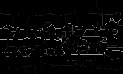
\includegraphics[width=0.30\textwidth]{figures/2008_000052_ucm.bmp.eps}
\caption{A UCM image from which a segmentation tree is derived.}
\label{fig:ucm}
\end{figure}

\begin{figure}
\centering
%\subfigure[]{
%\label{fig:treea}
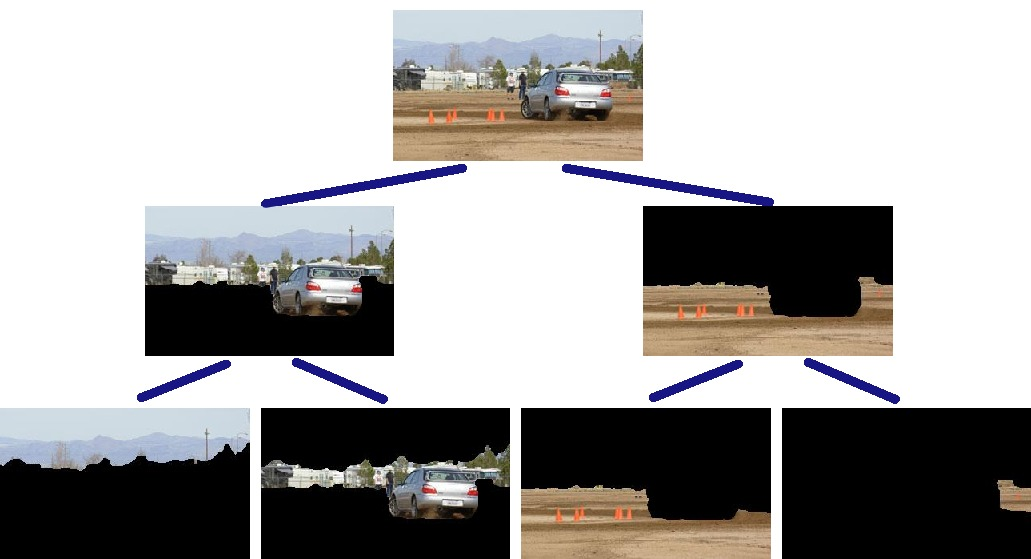
\includegraphics[width=0.45\textwidth]{figures/tree_additive.eps}
%}
%\subfigure[]{
%\label{fig:treeb}
%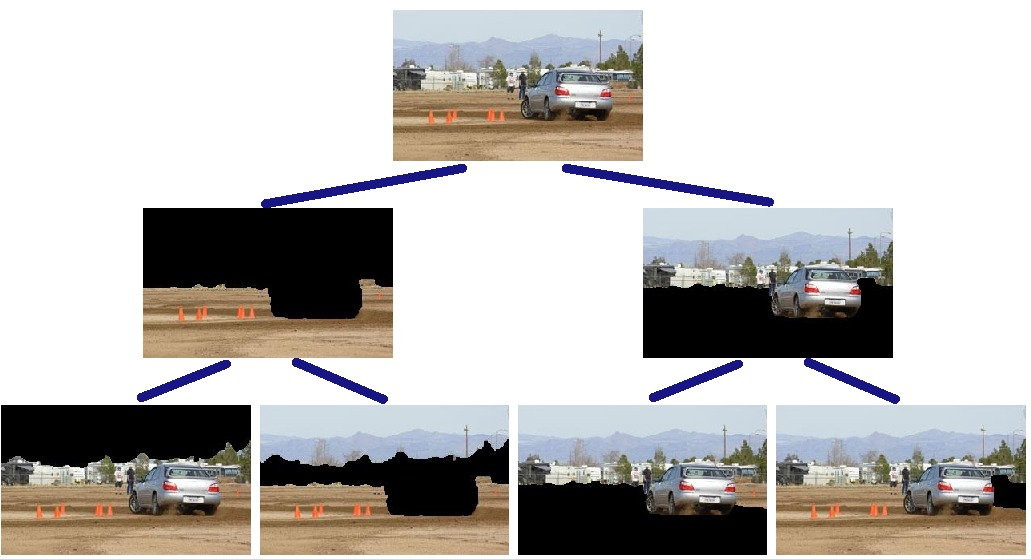
\includegraphics[width=0.45\textwidth]{figures/tree_subtractive.eps}
%}
\caption{The segmentation hierarchy used by the additive
and subtractive algorithms.  This tree was generated from the UCM
in figure \ref{fig:ucm}.}
\label{fig:tree}
\end{figure}

\subsection{Additive algorithm}
\label{ssec:additive}

This pruning algorithm is based on three observations. (1) At least
one node in the segmentation tree contrains the whole object. (This
is always true since the root node contains the whole image). (2) If
both parent node and child node have high confidence of containing
the object, the segmentation of the child node is more accurate than
that of the parent node. (3) Even if some node has high confidence
of containing the object, its segmentation can still be improved by
removing irrelevant children node. The details of the additive
algorithm is shown in algorithm \ref{alg:add_prune}.

The idea of the algorithm is to find the smallest discriminative
regions, either positive or negative. We combine all the smallest
positive regions while remove all the negative ones to form the
final segmentation. We use three threshold for the similarity
measure, $thre\_perf$, $thre\_pos$ and $thre\_neg$ which represent
perfect segment, positive segment and negative segment,
respectively. If the similarity is above $thre\_perf$, which means
the segmentation is perfect for the object, we cut all the nodes
below and return this segment. If the similarity is below
$thre\_neg$, which means the segment does not contain the object, we
cut all the nodes below and return NULL. If the similarity is
between $thre\_perf$ and $thre\_pos$, which means the node
definitely contains the object but the segmentation is not perfect
yet, we keep on checking its children nodes to refine the
segmentation. The final case is that the similarity is between
$thre\_pos$ and $thre\_neg$, which means we are not sure whether
there is an object in the node, so we just keep on searching its
children.

The object classification is based on the output of ADDITIVE\_PRUNE. If the output is not NULL, which means at least one node in the tree has similarity above $thre\_pos$, we think the object is detected in this image.


\begin{algorithm}
\begin{algorithmic}
  \STATE \textbf{input:}
  \STATE \hspace{3 mm} node $n$ in segmentation tree
  \STATE \hspace{3 mm} desired object model $obj\_model$
  \STATE \hspace{3 mm} threshold for perfect segment $thre\_perf$
  \STATE \hspace{3 mm} threshold for positive segment $thre\_pos$
  \STATE \hspace{3 mm} threshold for negative segment $thre\_neg$
  \STATE \textbf{output:}
  \STATE \hspace{3 mm} refined segment
  \STATE
  \STATE $sim=HI(obj\_model,n.conf)$
  \IF{$sim \ge thre\_perf$}
    \STATE return $n.segment$
  \ENDIF
  \IF{$sim \le thre\_neg$}
    \STATE return $NULL$
  \ENDIF
  \STATE $s'=NULL$
  \FOR{$i=1$ to $n.childNum$}
    \STATE s\{i\}=ADDITIVE\_PRUNE(n.children\{i\},obj\_model,...
    \STATE ... thre\_perf,thre\_pos,thre\_neg)
    \STATE s'=s'+s\{i\}
  \ENDFOR
  \IF{$sim\ge thre\_pos$ and $s'==NULL$}
    \STATE return n.segment
  \ELSE
    \STATE return s'
  \ENDIF
\end{algorithmic}
\caption{ADDITIVE\_PRUNE}
\label{alg:add_prune}
\end{algorithm}



\subsection{Subtractive algorithm}
\label{sec:sub}

The subtractive algorithm relies on the idea that if removing a region from
an image doesn't significantly affect the probability of the image containing
the object (which probability is obtained using the predicted attribute
distribution and is here used interchangably used with the term ``similarity'')
then that region can be safely removed in the final segmentation.
The algorithm itself is shown in algorithm \ref{alg:sub_prune}.

\begin{algorithm}
\begin{algorithmic}
  \STATE \textbf{global:}
  \STATE \hspace{3 mm} master mask $m_m$
  \STATE \textbf{input:}
  \STATE \hspace{3 mm} node $n$ in segmentation tree
  \STATE \hspace{3 mm} similarity $sim_{root}$ on root node
  \STATE \hspace{3 mm} factor $f$
  \STATE \textbf{output:}
  \STATE \hspace{3 mm} mask $m_m$
  \STATE
  \STATE $m_n$ := mask of $n$
  \STATE $r = m_{m} \cap \verb+~+ m_{n}$
  \STATE $pred\_model$ := predict attributes on image($r$)
  \STATE $sim=HI(obj\_model,pred\_model)$
  %\STATE $H_{pred}$ := predict attributes on image($m_n \cap m_m$)
  %\STATE $\displaystyle P_{pred} = \frac{H_{pattern} \cap H_{pred}}{H_{pattern} \cup H_{pred}}$
  \IF{$sim < f \cdot sim_{root}$}
    \FOR{$i=1$ to $n.childNum$}
      \STATE SUBTRACTIVE\_PRUNE(n.children\{i\},
      \STATE ...$sim_{root}$, $f$)
    \ENDFOR
    %\STATE SUBTRACTIVE\_PRUNE(n.children)
  \ELSE
    \STATE $m_m = m_m \cap \verb+~+ m_n$
  \ENDIF
\end{algorithmic}
\caption{SUBTRACTIVE\_PRUNE}
\label{alg:sub_prune}
\end{algorithm}

The algorithm begins at the root of the tree and predicts attributes.
This attribute distribution and its associated similarity $sim_{root}$
to the object's canonical distribution is taken to be
the standard for the image.  That is, any final segmentation should not have
significantly less similarity $sim$ than $sim_{root}$.  The algorithm traverses
the subtractive tree depth-first.  At each node, attributes are predicted for 
a region $r$.  
$r$ is obtained by taking the intersection of the master mask and the inverted
node mask ($r = m_{m} \cap \verb+~+ m_{n}$).  The intuition is this: the master mask is our current best guess at
the region that contains an object.  By taking the intersection, we effectively
subtract the node's region out.
We can then predict on the new region.  If 
there is no significant negative effect on the similarity as
compared to the standard, then we assume that we can safely prune off the node's
region without removing a part of the object..  If the
similarity was significantly affected, then we assume that the region
contains some part of the object and we allow it to remain.  But that 
doesn't mean that sub-regions might not be able to be pruned
out, so the procedure is called recursively, checking for smaller regions
that might be able to be pruned.

As mentioned, if the similarity score was not significantly affected by
predicting on the master mask with the region removed, then the region is
permanently removed from the master mask
and no recursive call is made.  This is important, because it means
that we can remove large chunks of the image wholesale and bypass predicting
on the node's posterity.
The runtime performance of the algorithm is dominated by the prediction step.
Thus the advantage of pruning large chunks early is highly beneficial to
the runtime of the algorithm.

$f$ is an important parameter that requires tuning.  Increasing $f$ makes the
algorithm more conservative, that is, less likely to apply removals.  Decreasing
$f$ makes it more liberal.  We found $f=0.9$ to be a reasonable value for most images.
Figure \ref{fig:f} shows results of adjusting $f$ between 0.9 and 1.0.

The subtractive algorithm knows nothing about the number of objects present
in the image.  It attempts to segment any object out into the final region.
This is evident in figure \ref{fig:sub1}.  The mobile homes in the background
have car attributes and thus are included in the final segmentation, even
though they take a far less prominent role in the unsegmented image.  Another
example is figure \ref{fig:truck}, where the two cars visually behind the truck
are segmented together with the truck.

\begin{figure}
\centering
\subfigure[]{
\label{fig:fa}
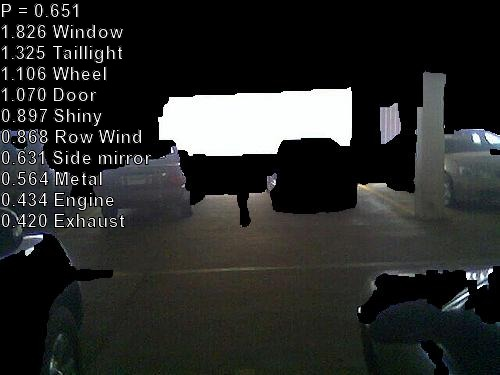
\includegraphics[width=0.22\textwidth]{figures/parking_0.9.eps}
}
\subfigure[]{
\label{fig:fb}
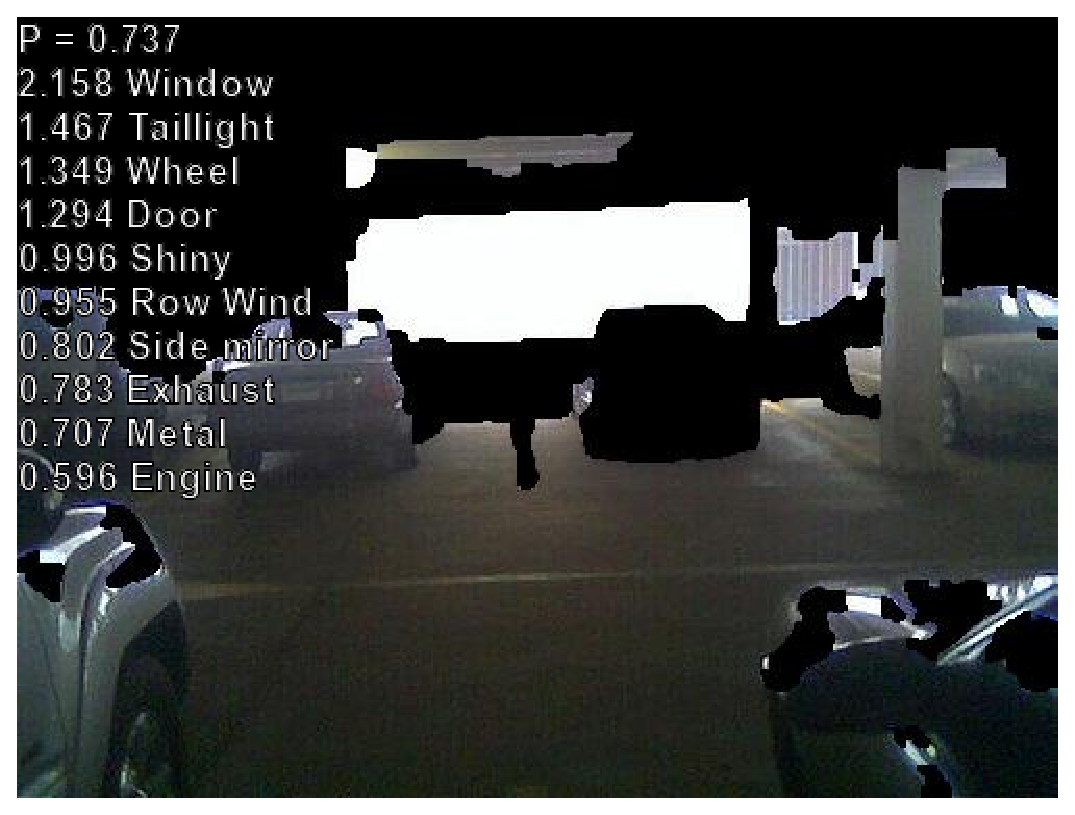
\includegraphics[width=0.22\textwidth]{figures/parking_1.0.eps}
} \caption{Result of adjusting the factor $f$ in the subtractive
algorithm. \subref{fig:fa} shows running the algorithm with $f=0.9$
and \subref{fig:fb} shows running the algorithm with $f=1.0$.  Note
that \subref{fig:fb} retains more of the cars, especially the two
closest on the right and left, but also has more false-positive
pixels, such as the ceiling region of the parking garage.}
\label{fig:f}
\end{figure}

\begin{figure}
\centering
\subfigure[]{
\label{fig:sub1a}
\includegraphics[width=0.22\textwidth]{figures/results/2008_000052.jpg.eps}
}
\subfigure[]{
\label{fig:sub1b}
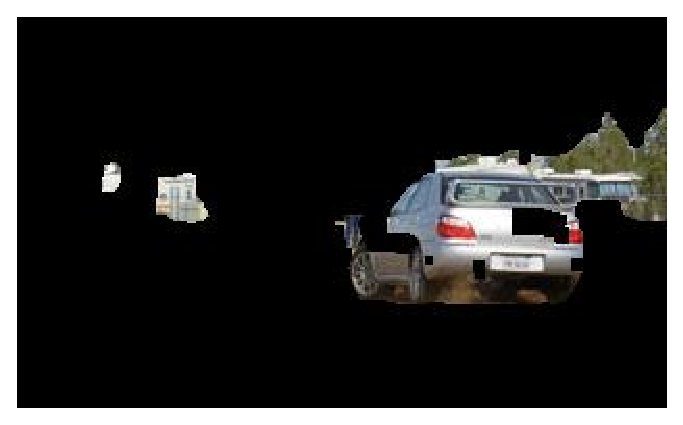
\includegraphics[width=0.22\textwidth]{figures/2008_000052_1.00.jpg.eps}
} \caption{Subtractive segmentation on an image with multiple objects.
An observer may not even notice the trailer homes in the background in
the original image \subref{fig:sub1a},
but the segmentation includes a portion of them in the final segmentation \subref{fig:sub1b}.
Subtractive segmentation attempts to segment all objects present
in the image.}
\label{fig:sub1}
\end{figure}

%-------------------------------------------------------------------------------
% experimental results
%-------------------------------------------------------------------------------
\section{Experimental results}
\label{sec:results}


In this section, we evaluate our attribute based object classification
and segmentation algorithms. We also analyze the advantages and 
disadvantages of our algorithms.\\

\subsection{Dataset}
\label{ssec:dataset}

We used the Pascal2008 dataset for both training and testing. This dataset contains real life
images which are generally difficult to classify. 
For training and testing of classification and
segmentation we used the pascal2008 training and validation sets, respectively.
The objects are labeled
by bounding boxes -- unfortunately accurate segmentations are not available
with this dataset.  The attribute
annotations used in \cite{farhadi09} are freely available and we
used them for both training and testing. Three classes are used in this experiment, including car,
airplane and horse. We used 328 test images, with 150 car, 103 airplane and 93 horse. 
Note that any given image may
contain multiple objects in multiple classes.\\

\subsection{Measure}
\label{ssec:measure}

For object classification, we use precision and recall to measure the performance. 
For segmentation, we use the ratio of intersection and union of the prediction and 
groundtruth as the measure of precision. The segmentation
precision is calculated with
\[ V(M_{groundtruth},M_{pred}) = \frac{|M_{groundtruth} \cap M_{pred}|}{|M_{groundtruth} \cup M_{pred}|} \]
where $M_{groundtruth}$ is the groundtruth mask calculated from the
bounding boxes stored with the annotations and $M_{pred}$ is the
predicted segmentation mask.  We of course recognize that the
bounding boxes are not a good measure of segmentation truth, but
it's the best we have available.\\

\subsection{Classification}
\label{ssec:classification}

Table \ref{table:aresults} shows the classification results comparing the proposed method with 
the other three baseline methods. LowFea means that we use the low level feature to train and test 
the object classification directly. Att1 means that we use the attribute distribution as the feature,
but we only test it in the whole image without segmentation. Random means random prediction. Add is our
proposed algorithm with additive pruning. The proposed algorithm has the highest precision comparing 
with the other baselines, while the recall is a little lower than LowFea. Figure \ref{fig:roc_class} 
shows the ROC curve for each class and the average.

The subtractive algorithm is not included in classification results as it performs no
object detection or classification and assumes that the given object is present
in the image.


\begin{table}
\centering
\begin{tabular}{|l|l|l|}
\hline Methods & Precision(\%) & Recall(\%) \\
\hline LowFea  & 55.97 & 70.96 \\
\hline Att1    & 51.89 & 51.89 \\
\hline Random  & 35.19 & 50.00 \\
\hline Add     & 60.82 & 54.06 \\
\hline
\end{tabular}
\caption{Object classification results of three baseline methods and the proposed additive algorithm.}
\label{table:aresults}
\end{table}


\begin{figure}
\centering
\includegraphics[width=0.5\textwidth]{figures/add_res/roc_class.png.eps}
\caption{Result of adjusting the factor $f$ in the subtractive
algorithm. \subref{fig:fa} shows running the algorithm with $f=0.9$
and \subref{fig:fb} shows running the algorithm with $f=1.0$.  Note
that \subref{fig:fb} retains more of the cars, especially the two
closest on the right and left, but also has more false-positive
pixels, such as the ceiling region of the parking garage.}
\label{fig:roc_class}
\end{figure}


\subsection{Segmentation}
\label{ssec:segmentation}

Figure \ref{fig:roc_seg} shows the segmentation precision of additive pruning 
versus the false positive rate of object classification. The segmentation precision
is in the range of $20\%$ to $50\%$. Some of the segmentation results are shown in 
Figure \ref{fig:car_good_results},\ref{fig:car_bad_results},\ref{fig:aeroplane_good_results},\ref{fig:aeroplane_bad_results},\ref{fig:horse_good_results},\ref{fig:horse_bad_results}.  Again, the subtractive algorithm doesn't produce
analogous results as it performs no classification.

Figure \ref{fig:sub_seg_prec} shows a plot of segmentation precision against 
attribute similarity for the subtractive algorithm.  As discussed in section 
\ref{sec:sub}, the original image (the root node of the segmentation tree)
is given an attribute similarity score compared to the canonical.  This score
drives the subtractive algorithm, and the final segmentation can have a score
no lower than $f\cdot sim_{root}$.  The figure shows the final segmentation's
similarity score along the x-axis and the segmentation precision on the y-axis.
As expected, as the similarity score (or confidence in the existence of the
object) increases, the quality of the segmentation also increases.

Figures \ref{fig:car_good_results} and \ref{fig:car_bad_results} show the
segmentations of car images by both additive and subtractive pruning
algorithms. These show that it is somewhat unclear which pruning algorithm
gives the best performance (although a precision measure could be used if we
had better ground truth data).  But the results show some interesting patterns.
In general, the subtractive algorithm tends to produce more fragmented results
than the additive.  This is because the pruning algorithm searches all the way
to the bottom of the segmentation tree searching for regions that can be removed.
There are various techniques that could fix this, such as doing some kind of
confidence propagation from a ``good'' node to its descendents, in a similar
spirit to \cite{borenstein04}.  But while the additive algorithm does tend
to retain large portions of the car, it is often far too conservative, as
can be seen in figure \ref{fig:car_bad_results}.  Of course, this can be 
fixed by adjusting the threshold parameters, but this puts too much responsibility
on parameter selection for specific cases and causes it to not generalize well.

Figures \ref{fig:aeroplane_good_results}, \ref{fig:aeroplane_bad_results} and 
\ref{fig:horse_good_results}, \ref{fig:horse_bad_results} show some good and bad 
segmentation results of the additive algorithm on airplane and horse classes. Because of the
high complexity of the subtractive algorithm, we did not run it on these two classes. 
Figures \ref{fig:aeroplane_good_results} and \ref{fig:horse_good_results} show some
of the more impressive segmentations.  The third column in each figure shows that
the algorithm segments out multiple objects at the same time.

Figures \ref{fig:aeroplane_bad_results} and \ref{fig:horse_bad_results} show results
that either miss part of the object or contain a lot of background.  Extreme cases,
such as the second image in \ref{fig:horse_bad_results} mask out the object of interest
(horse, in this case) and almost nothing else.  These errors are cause by two things:
first, the additive algorithm currently does not use all levels in the segmentation tree,
as it would have made testing take prohibitively long.
Another problem with searching deep in the tree is that when the segments are too small, 
the attribute detection is nearly random, because the small regions 
don't have enough points to represent their properties. Second, the training of attributes based on
bounding boxes is not accurate, because of many background pixels can be included in the bounding boxes. 
This is especially obvious to the horse images, since horses are far from having a convex shape. 
All the segmented images in figure \ref{fig:horse_bad_results} contains grass or trees, especially the 
left one which only contains grass. These images imply that the grass and tree models are actually
included in the horse model.\\  


\begin{figure}
\centering
\includegraphics[width=0.5\textwidth]{figures/add_res/roc_seg.png.eps}
\caption{Result of adjusting the factor $f$ in the subtractive
algorithm. \subref{fig:fa} shows running the algorithm with $f=0.9$
and \subref{fig:fb} shows running the algorithm with $f=1.0$.  Note
that \subref{fig:fb} retains more of the cars, especially the two
closest on the right and left, but also has more false-positive
pixels, such as the ceiling region of the parking garage.}
\label{fig:roc_seg}
\end{figure}

\begin{figure}
\centering
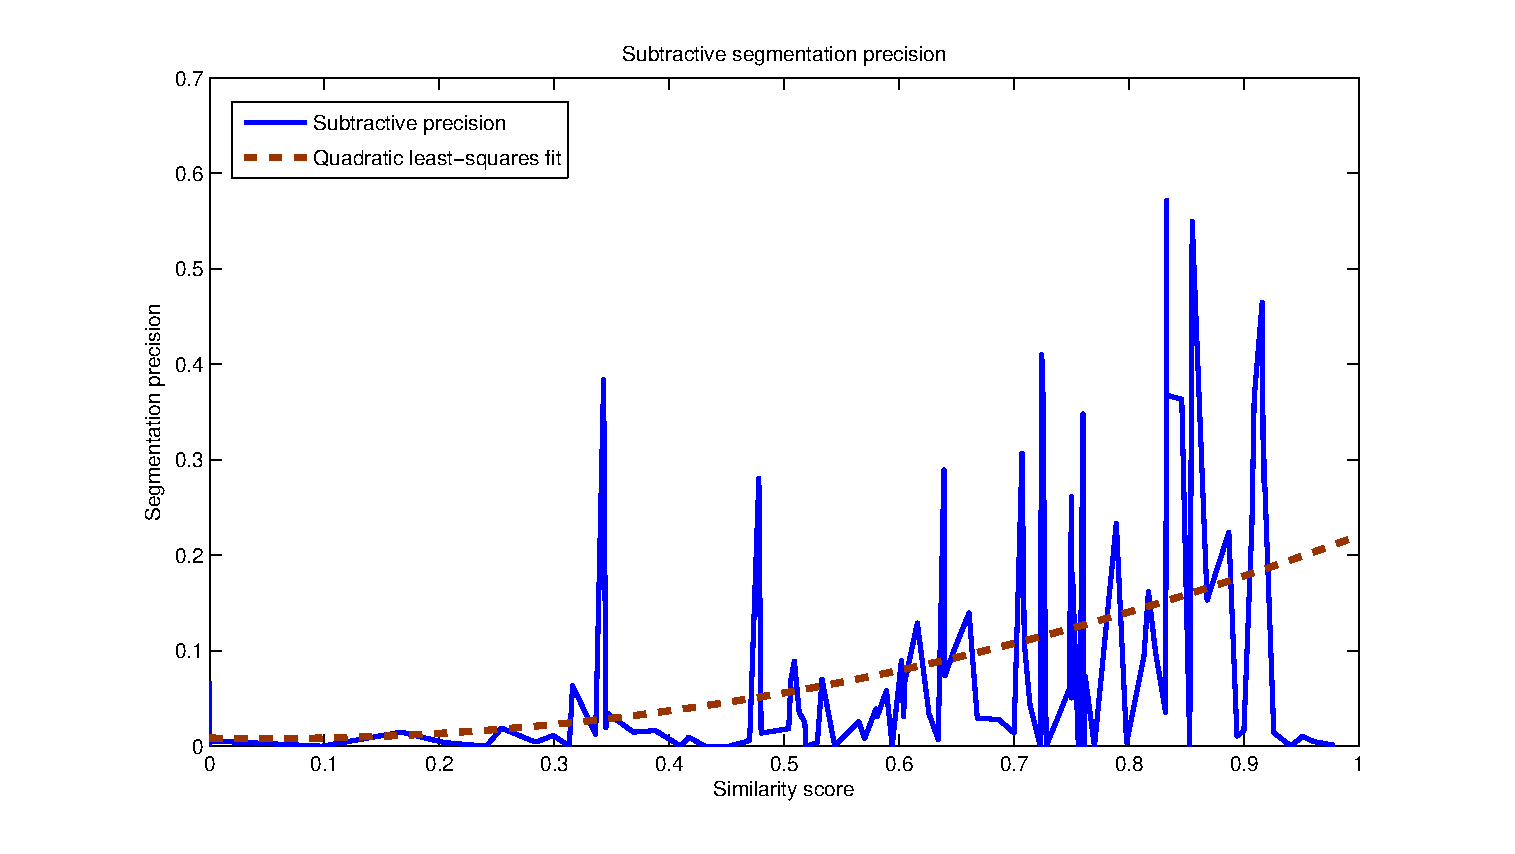
\includegraphics[width=0.5\textwidth]{figures/SubSegPrec.eps}
\caption{Graph of the precision of the subtractive segmentation
algorithm against confidence, or attribute similarity.  Despite
the noise, there is an upward trend in the precision
as the similarity score increases, as shown by the 
quadratic least-squares fit.}
\label{fig:sub_seg_prec}
\end{figure}



%\begin{figure*}[p]
%\centering
%\begin{tabular}{ p{4cm} p{4cm} p{4cm} p{4cm} }
%\includegraphics[width=3.95cm]{figures/results/2008_000052.jpg.eps} &
%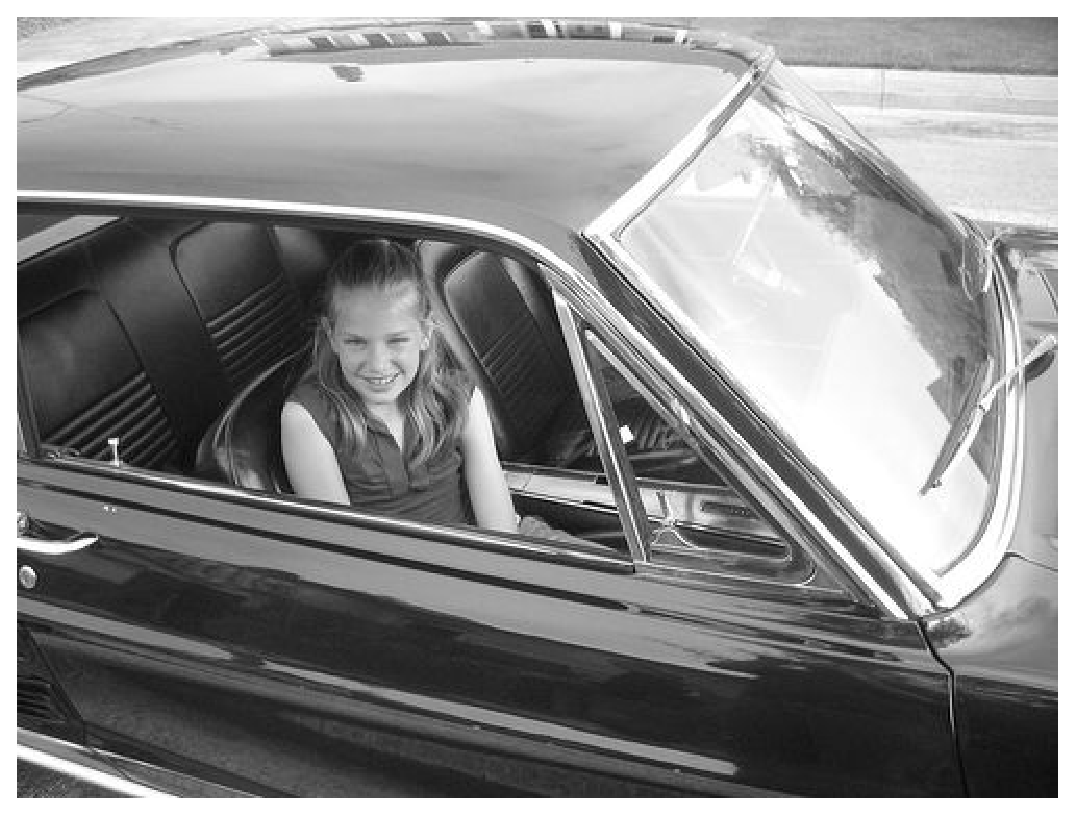
\includegraphics[width=3.95cm]{figures/results/2008_000828.jpg.eps} &
%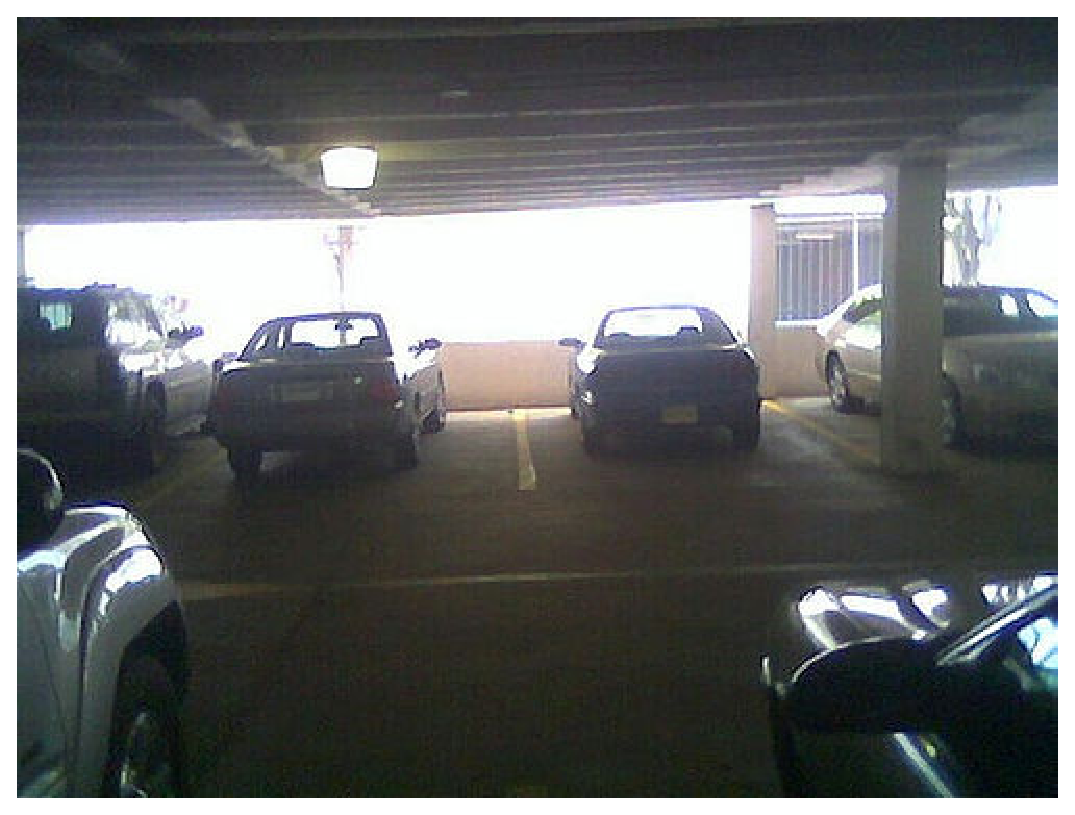
\includegraphics[width=3.95cm]{figures/results/2008_000952.jpg.eps} &
%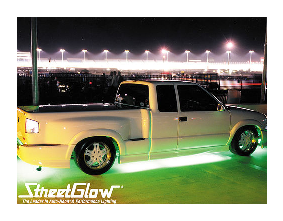
\includegraphics[width=3.95cm]{figures/results/2008_002198.jpg.eps} \\
%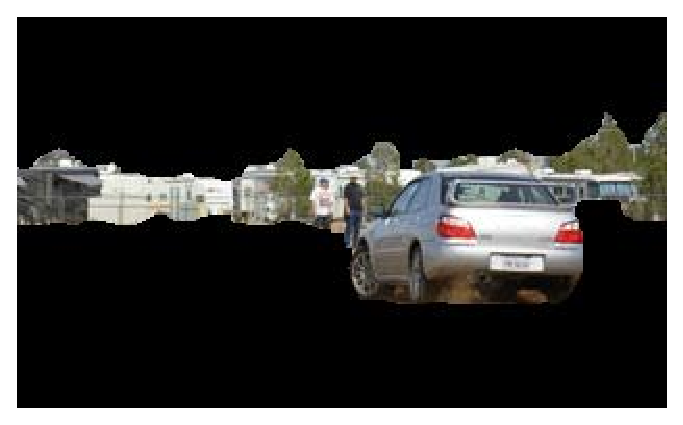
\includegraphics[width=3.95cm]{figures/results/a2008_000052.jpg.eps} &
%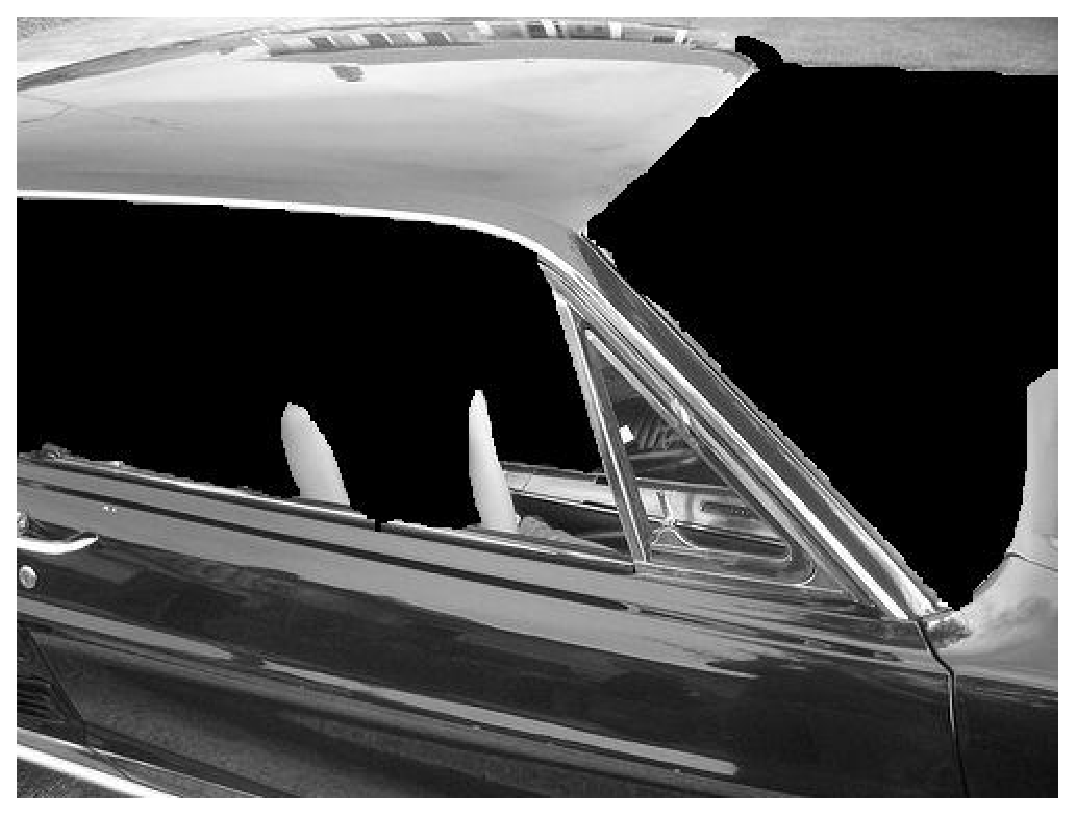
\includegraphics[width=3.95cm]{figures/results/a2008_000828.jpg.eps} &
%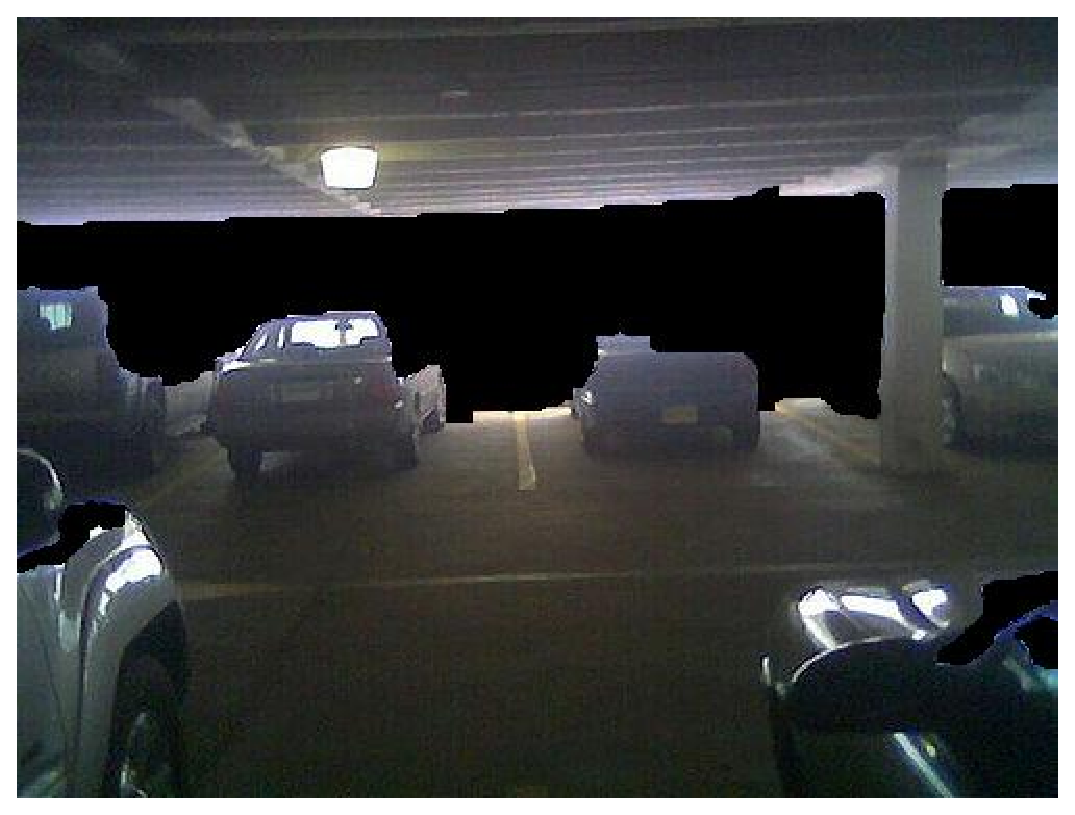
\includegraphics[width=3.95cm]{figures/results/a2008_000952.jpg.eps} &
%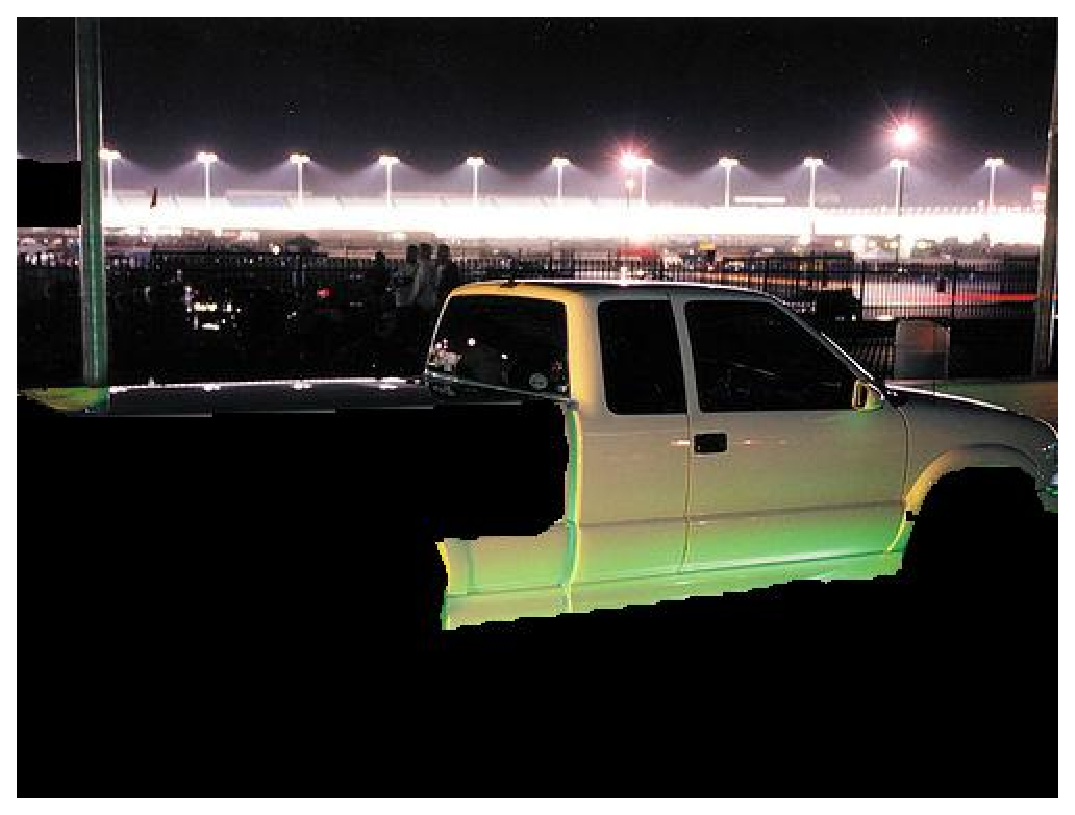
\includegraphics[width=3.95cm]{figures/results/a2008_002198.jpg.eps} \\
%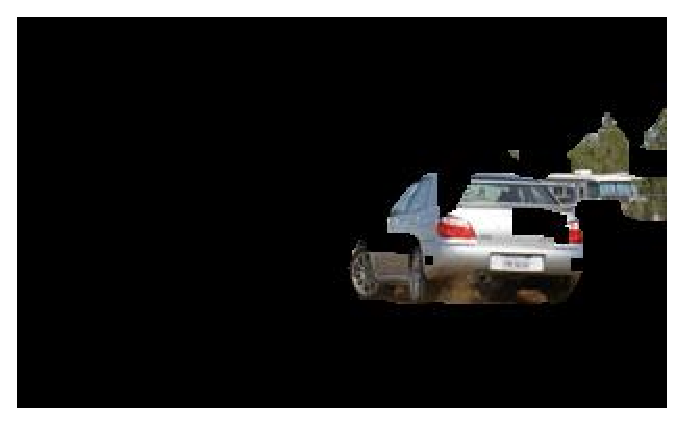
\includegraphics[width=3.95cm]{figures/results/b2008_000052.jpg.eps} &
%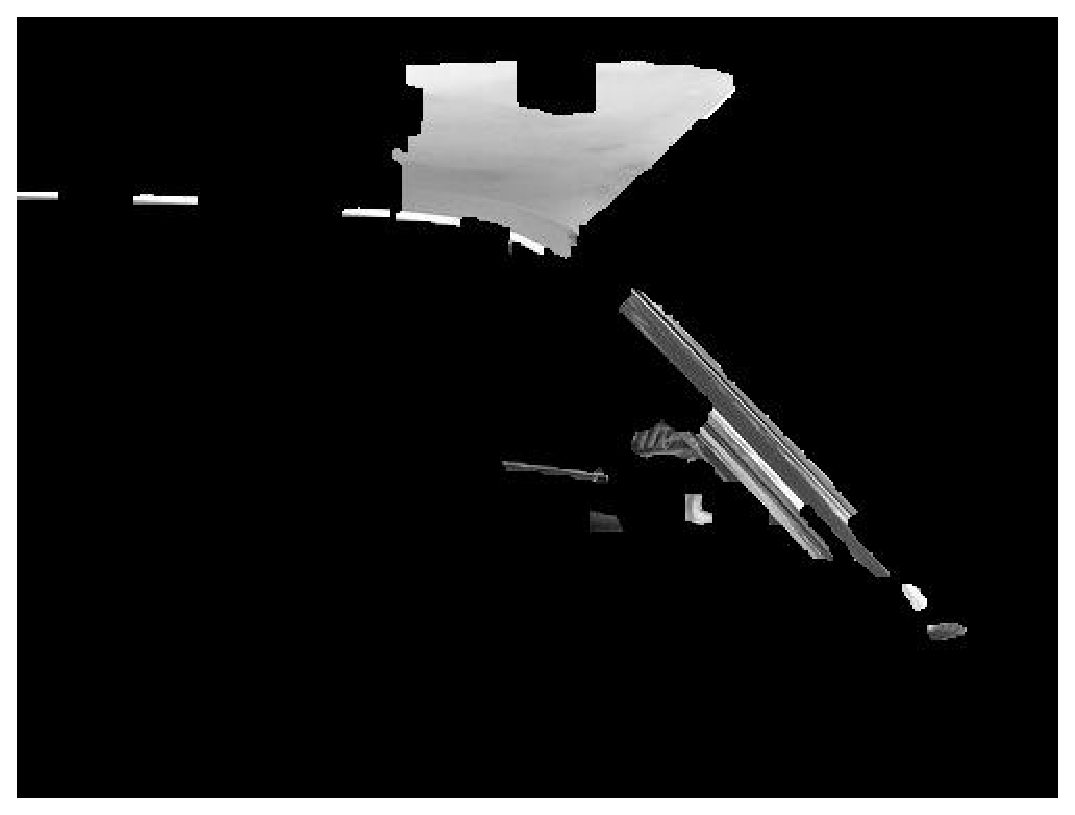
\includegraphics[width=3.95cm]{figures/results/b2008_000828.jpg.eps} &
%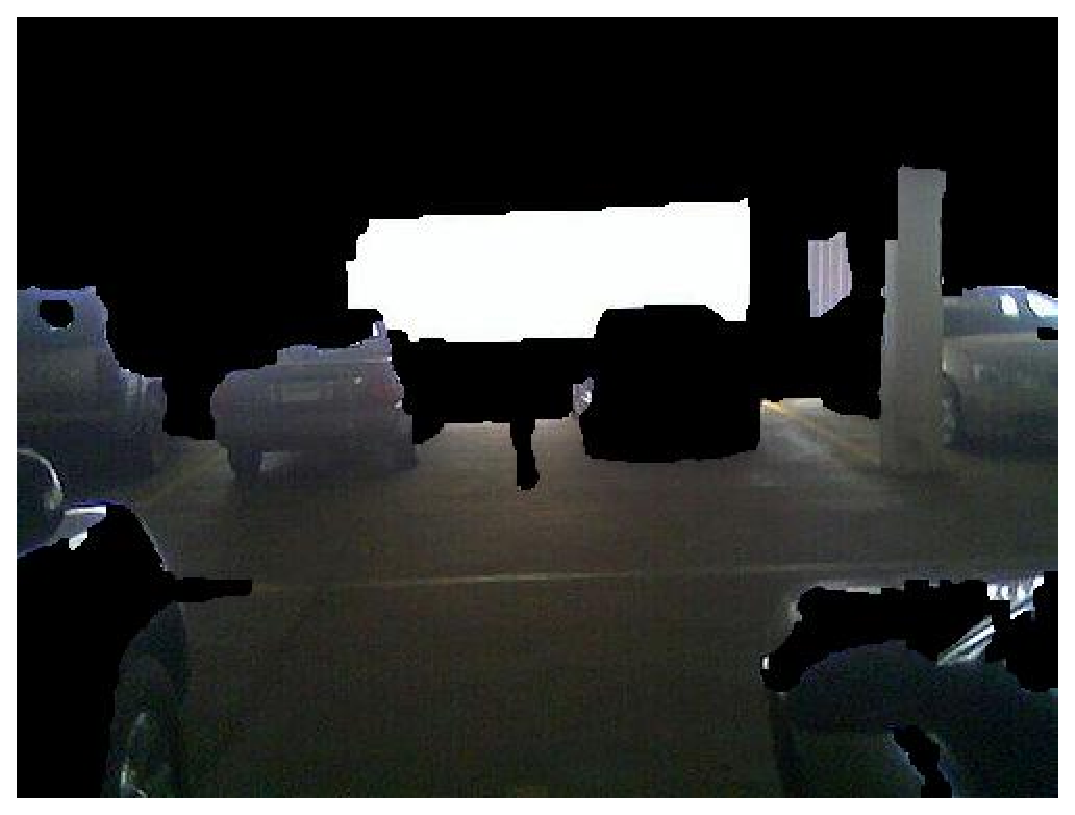
\includegraphics[width=3.95cm]{figures/results/b2008_000952.jpg.eps} &
%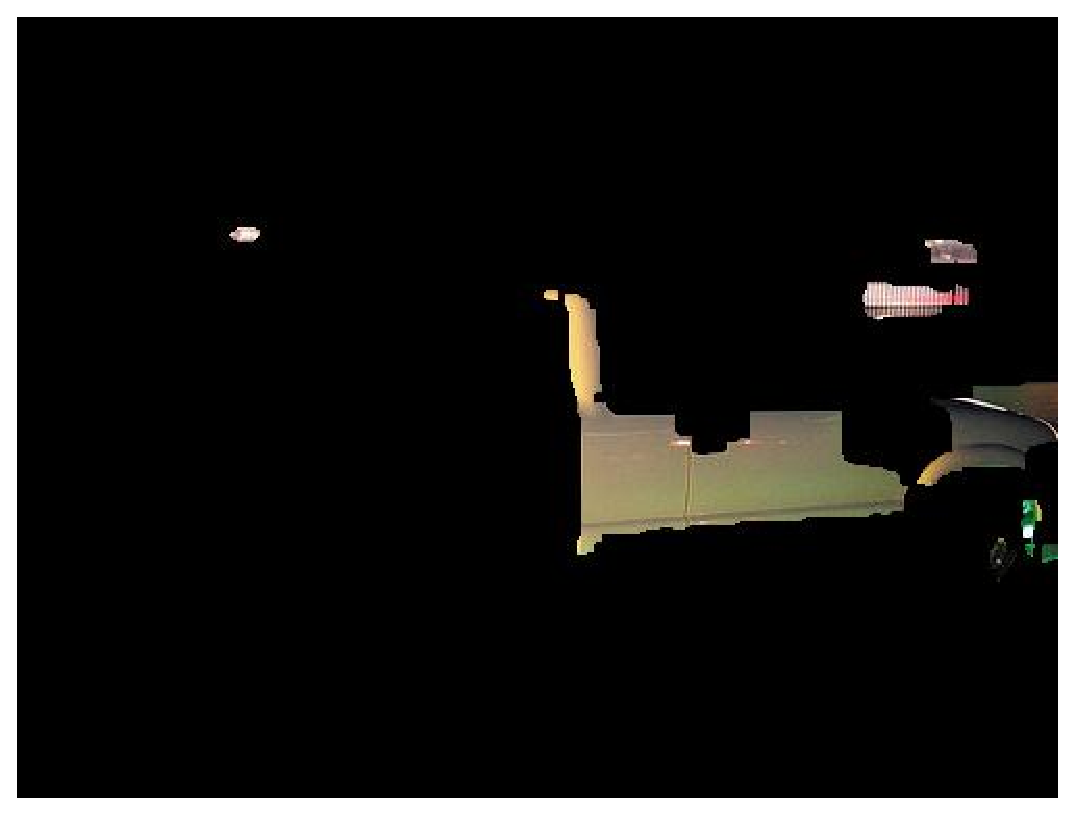
\includegraphics[width=3.95cm]{figures/results/b2008_002198.jpg.eps} \\
%\end{tabular}
%\caption{Selected results from segmentation of cars from the Pascal2008
%dataset.  The first row shows the original image.  The second row shows
%the best segmentation from the additive algorithm.  The third row shows
%the segmentation from the subtractive algorithm with $f=0.9$.}
%\label{fig:good_results}
%\end{figure*}

%\begin{figure*}[p]
%\centering
%\begin{tabular}{ p{4cm} p{4cm} p{4cm} p{4cm} }
%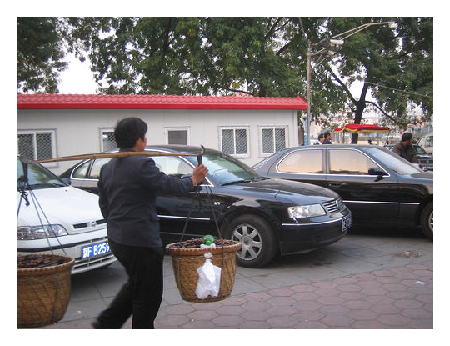
\includegraphics[width=3.95cm]{figures/results/2008_002483.jpg.eps} &
%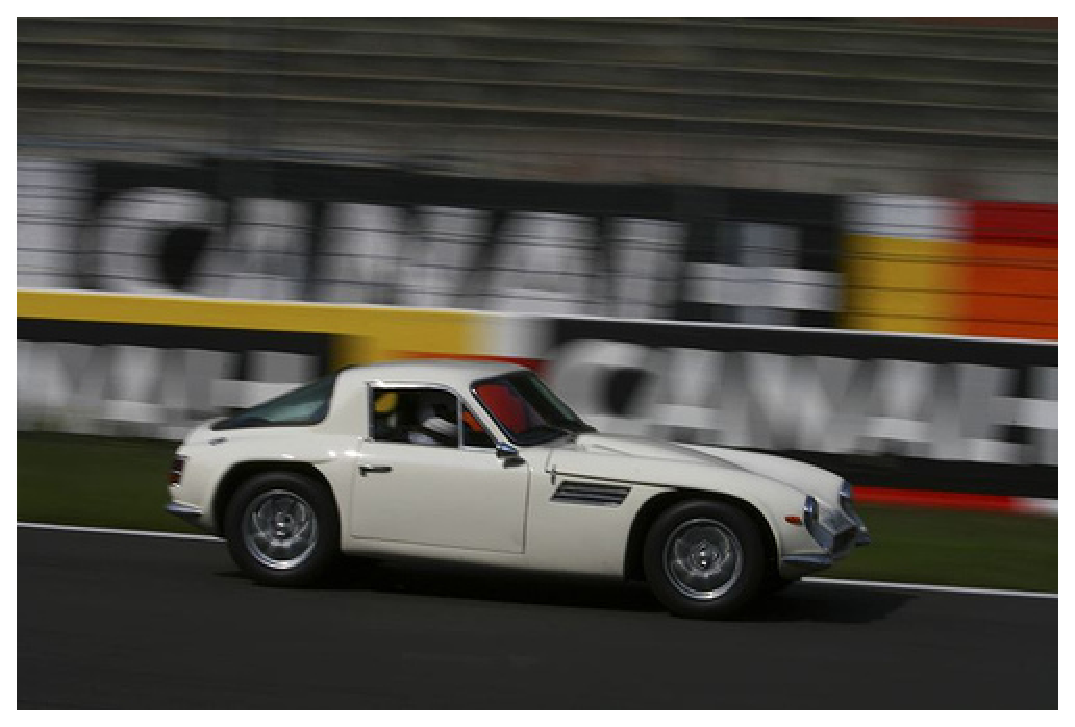
\includegraphics[width=3.95cm]{figures/results/2008_007466.jpg.eps} &
%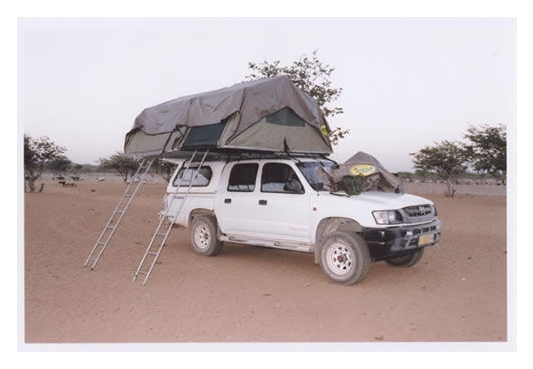
\includegraphics[width=3.95cm]{figures/results/2008_005378.jpg.eps} &
%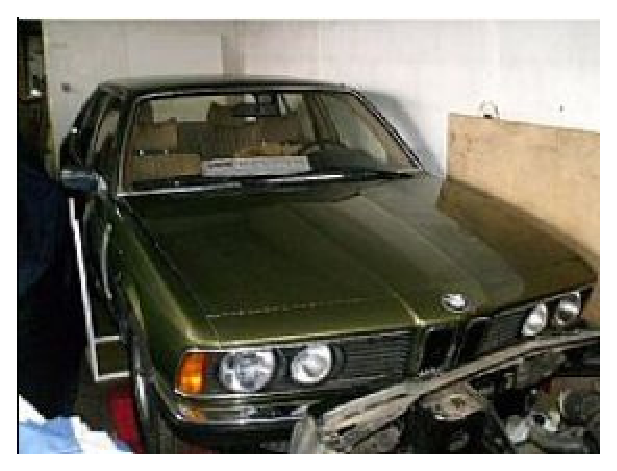
\includegraphics[width=3.95cm]{figures/results/2008_007529.jpg.eps} \\
%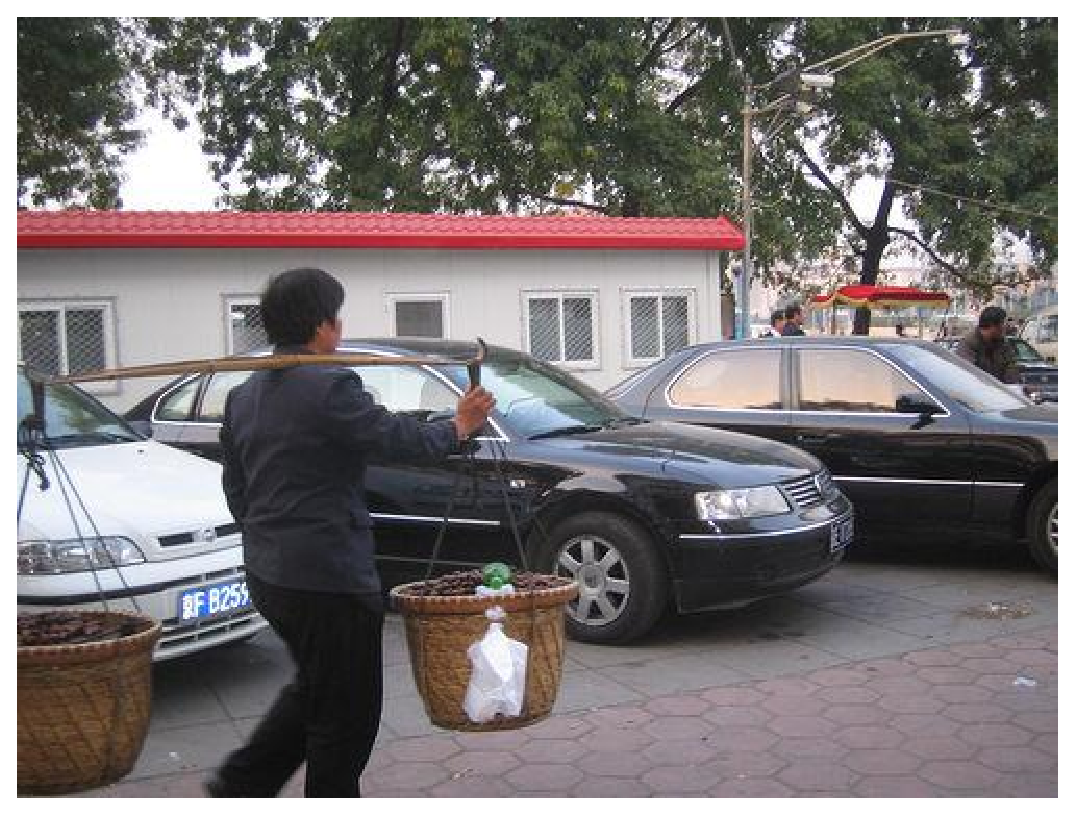
\includegraphics[width=3.95cm]{figures/results/a2008_002483.jpg.eps} &
%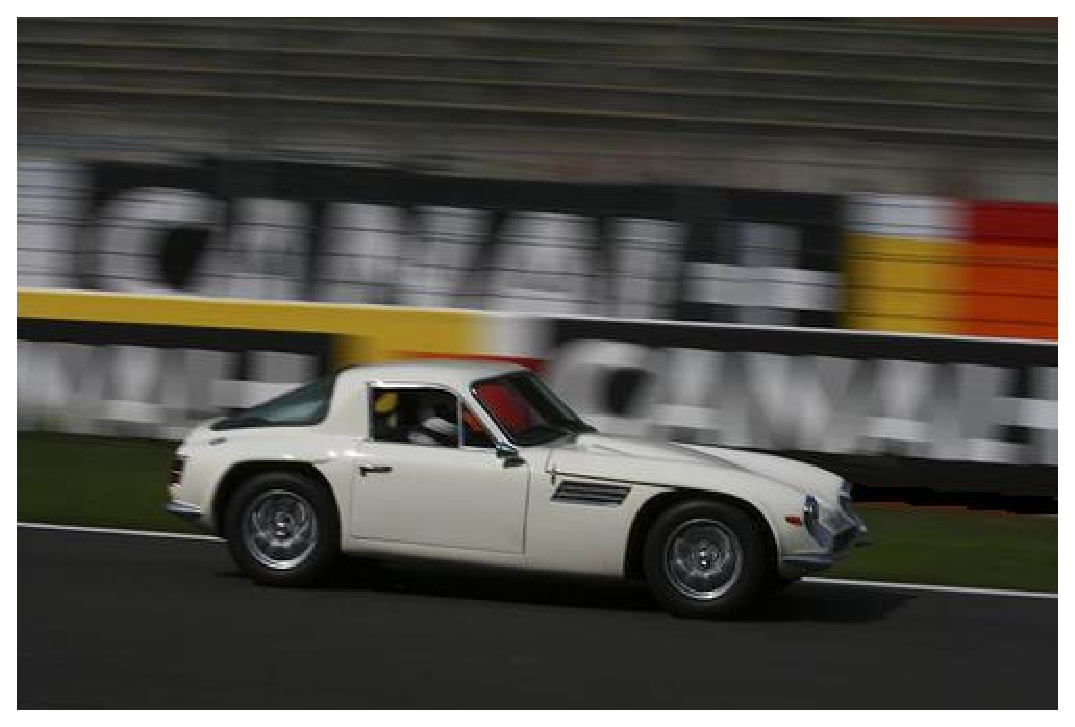
\includegraphics[width=3.95cm]{figures/results/a2008_007466.jpg.eps} &
%\includegraphics[width=3.95cm]{figures/results/a2008_005378.jpg.eps} &
%Car not detected &
%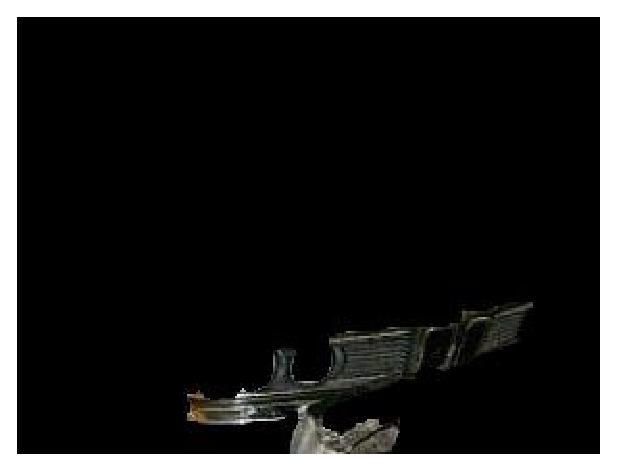
\includegraphics[width=3.95cm]{figures/results/a2008_007529.jpg.eps} \\
%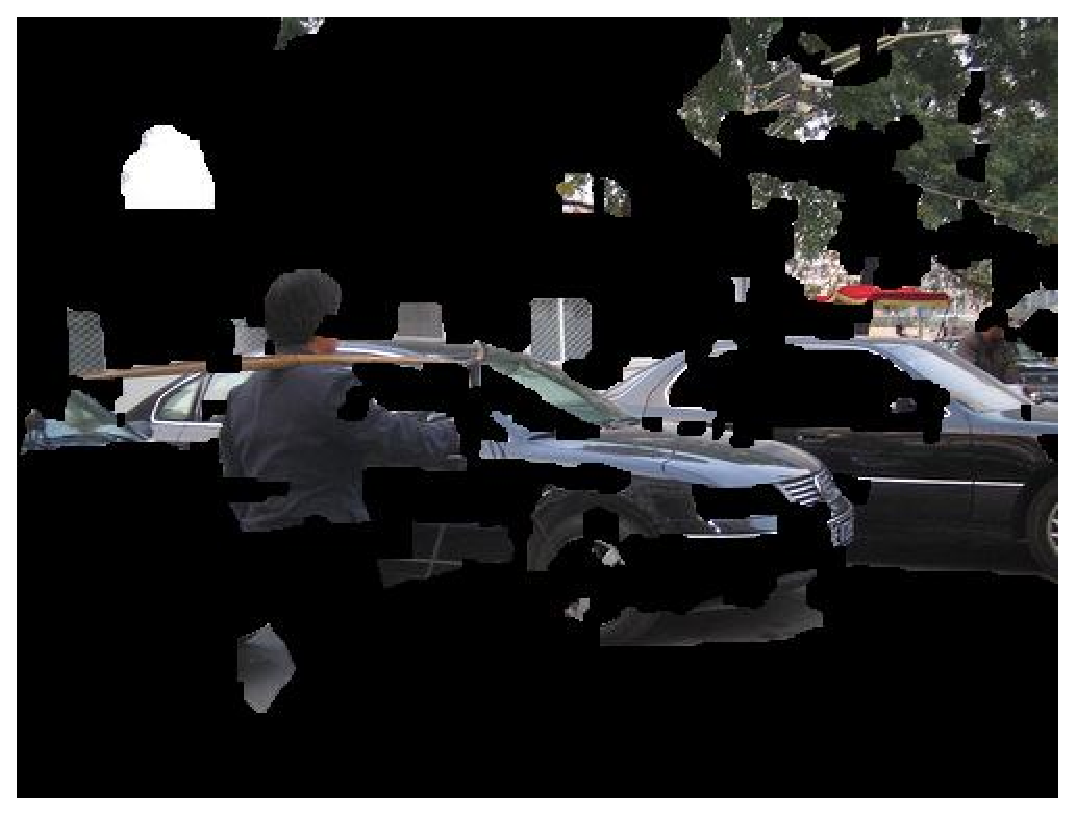
\includegraphics[width=3.95cm]{figures/results/b2008_002483.jpg.eps} &
%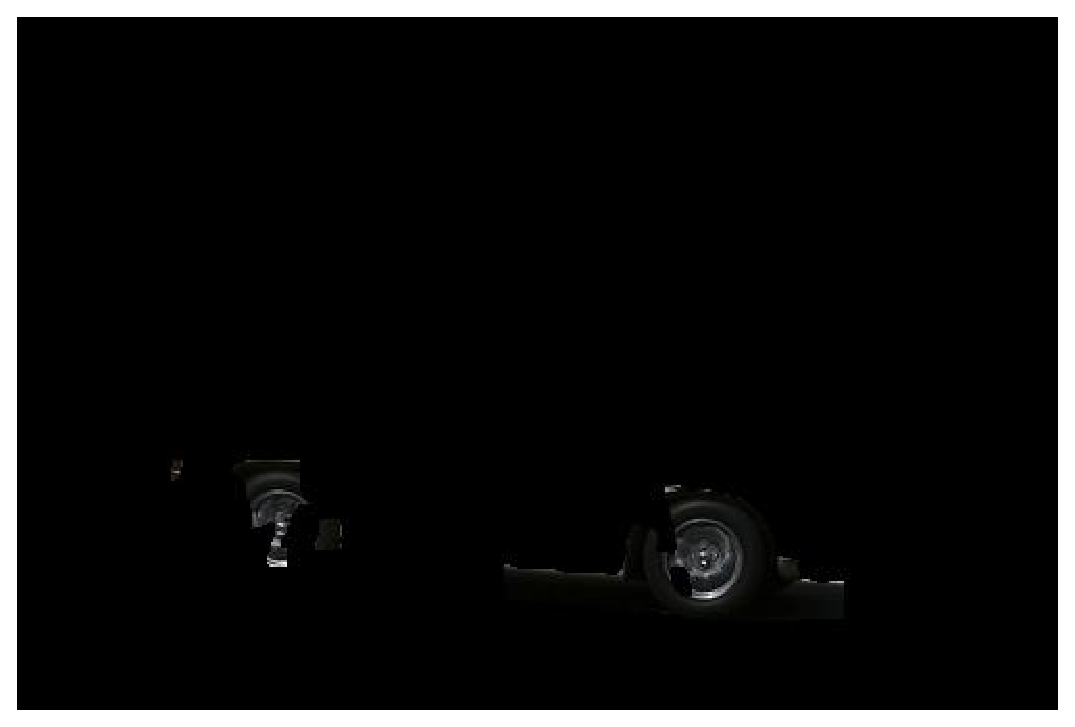
\includegraphics[width=3.95cm]{figures/results/b2008_007466.jpg.eps} &
%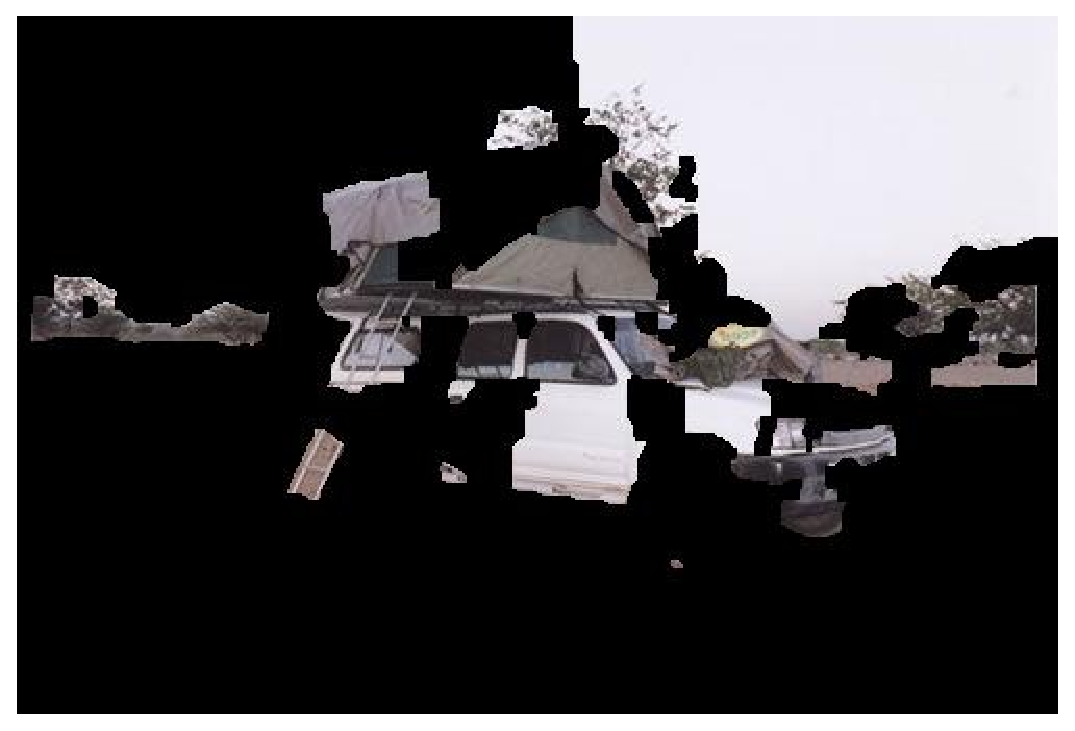
\includegraphics[width=3.95cm]{figures/results/b2008_005378.jpg.eps} &
%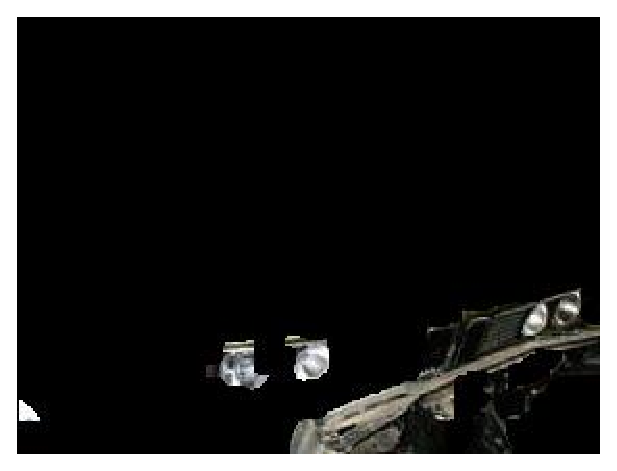
\includegraphics[width=3.95cm]{figures/results/b2008_007529.jpg.eps} \\
%\end{tabular}
%\caption{Selected results from segmentation of cars from the Pascal2008
%dataset.  The first row shows the original image.  The second row shows
%the best segmentation from the additive algorithm.  The third row shows
%the segmentation from the subtractive algorithm with $f=0.9$.}
%\label{fig:bad_results}
%\end{figure*}


\begin{figure*}[p]
\centering
\begin{tabular}{ p{3cm} p{3cm} p{3cm} p{3cm} }
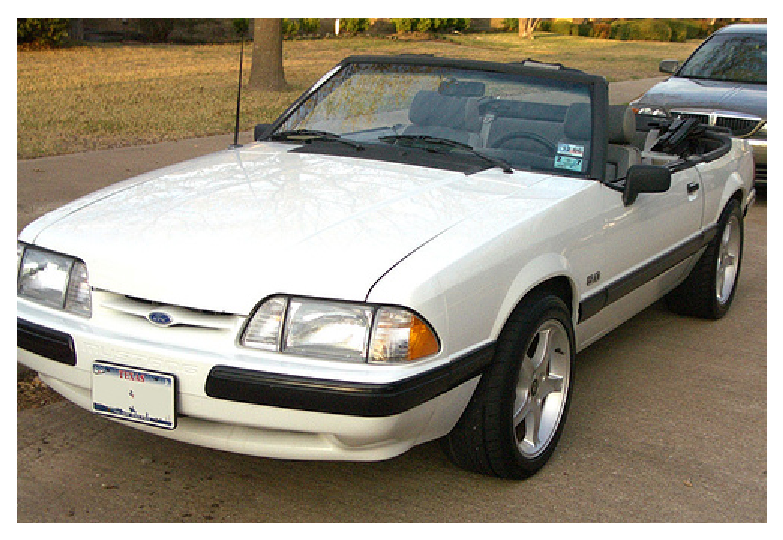
\includegraphics[width=2.95cm]{figures/add_res/car/2008_007064.jpg.eps} &
\includegraphics[width=2.95cm]{figures/add_res/car/2008_000052.jpg.eps} &
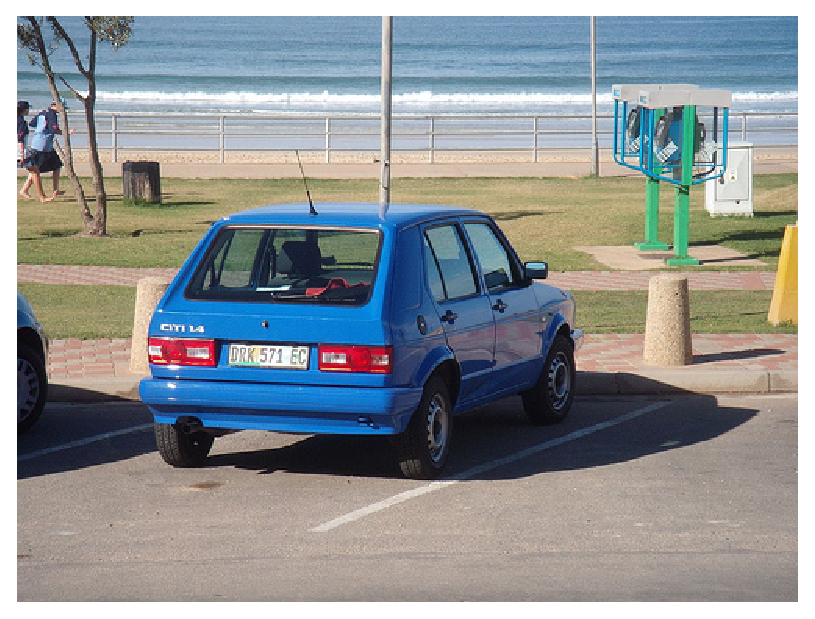
\includegraphics[width=2.95cm]{figures/add_res/car/2008_007171.jpg.eps} &
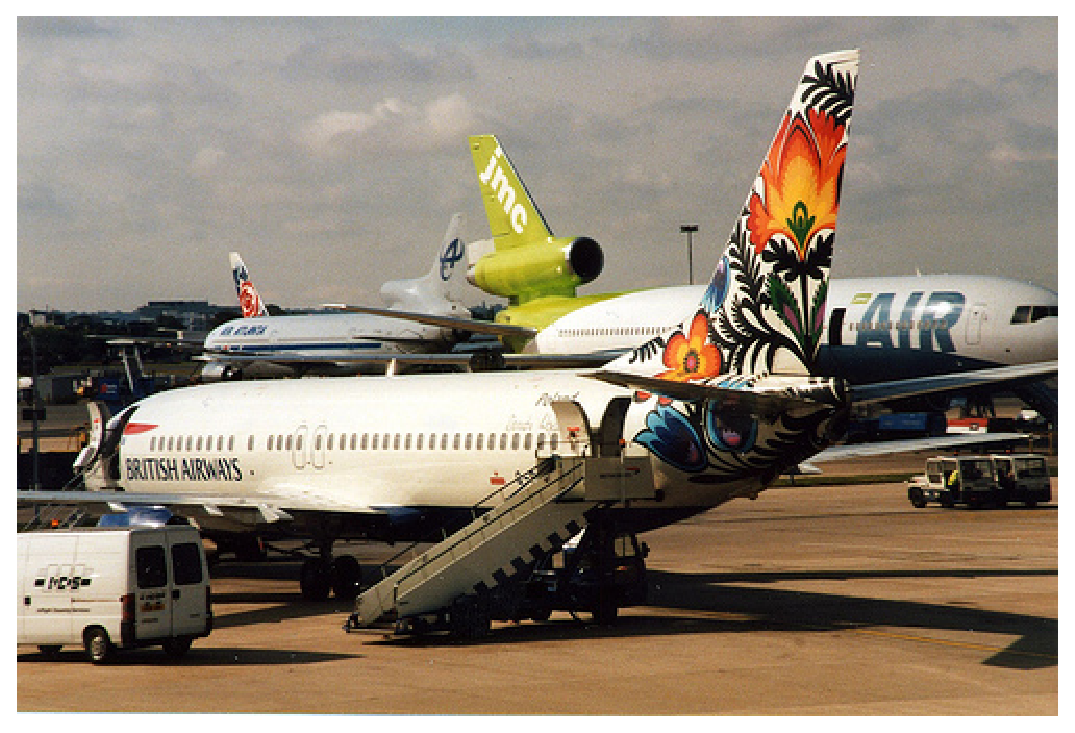
\includegraphics[width=2.95cm]{figures/add_res/car/2008_000251.jpg.eps} \\

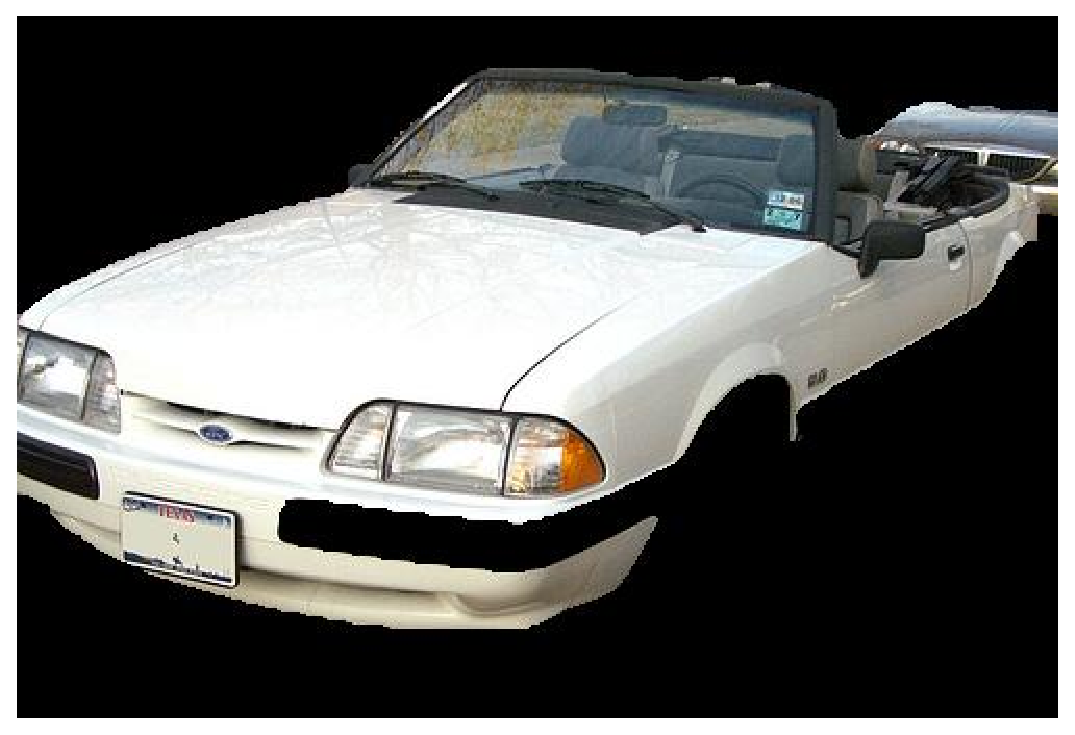
\includegraphics[width=2.95cm]{figures/add_res/car/2008_007064.jpg_1_good.jpg.eps} &
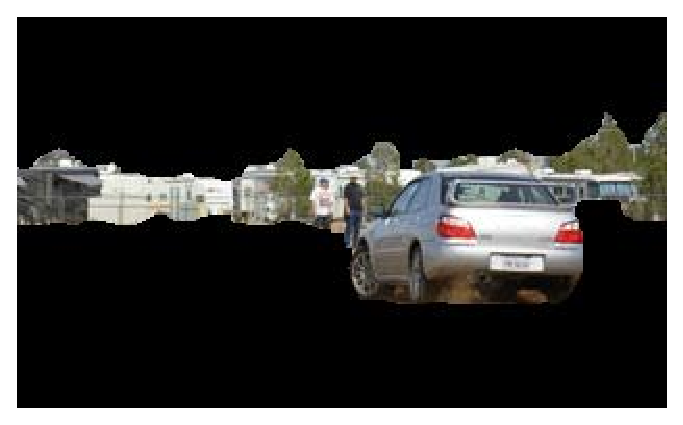
\includegraphics[width=2.95cm]{figures/add_res/car/2008_000052.jpg_1_good.jpg.eps} &
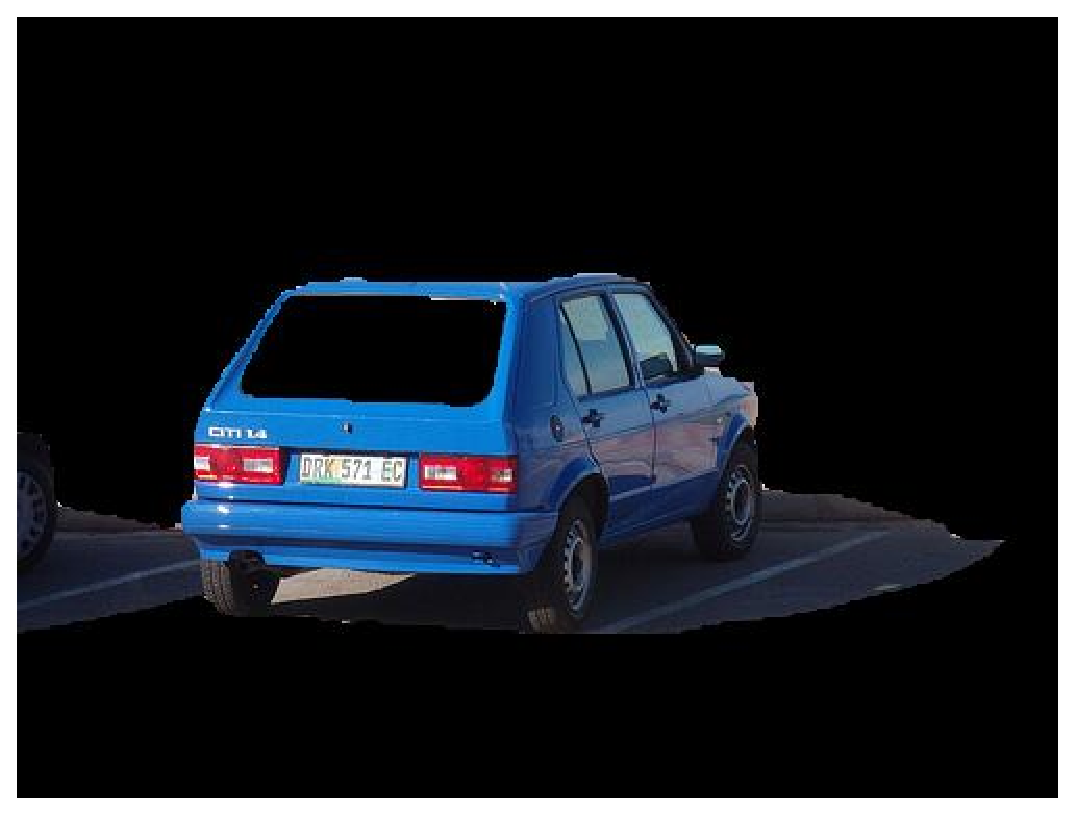
\includegraphics[width=2.95cm]{figures/add_res/car/2008_007171.jpg_1_good.jpg.eps} &
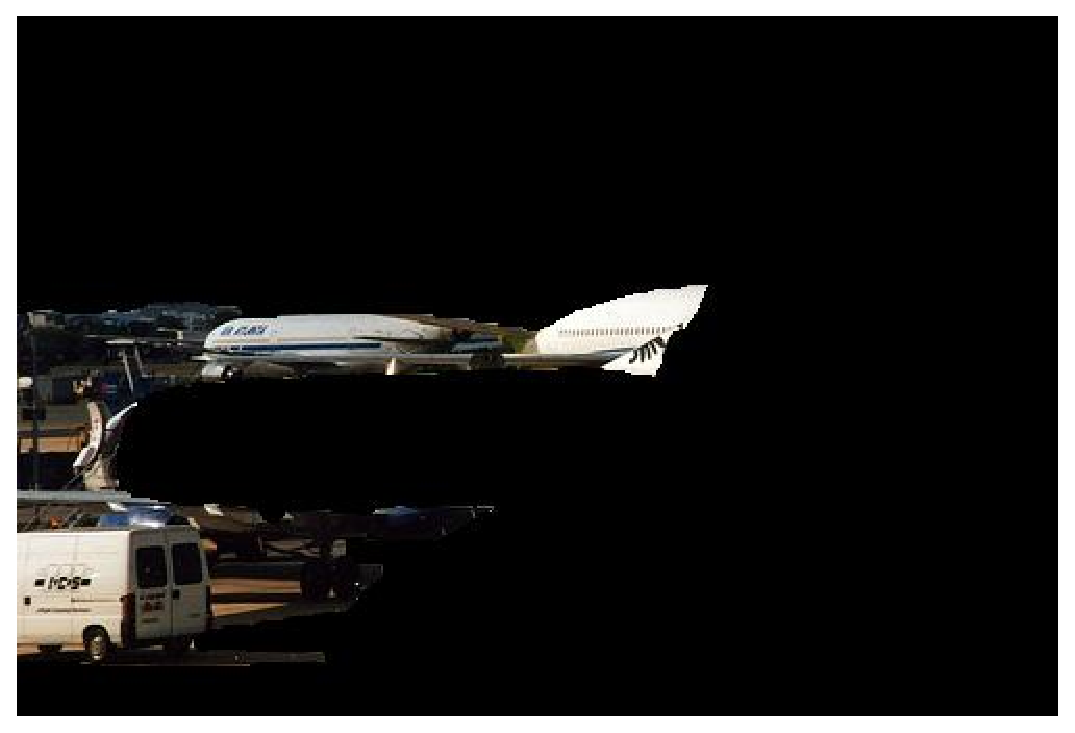
\includegraphics[width=2.95cm]{figures/add_res/car/2008_000251.jpg_1_good.jpg.eps} \\

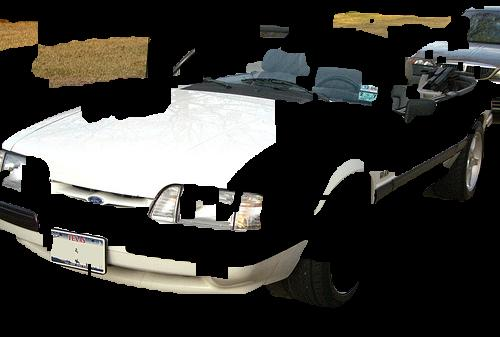
\includegraphics[width=2.95cm]{figures/sub_results/2008_007064_1_bad_sub.jpg.eps} &
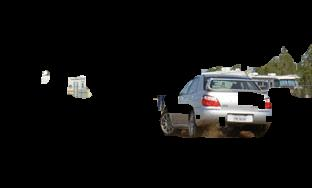
\includegraphics[width=2.95cm]{figures/sub_results/2008_000052_1_bad_sub.jpg.eps} &
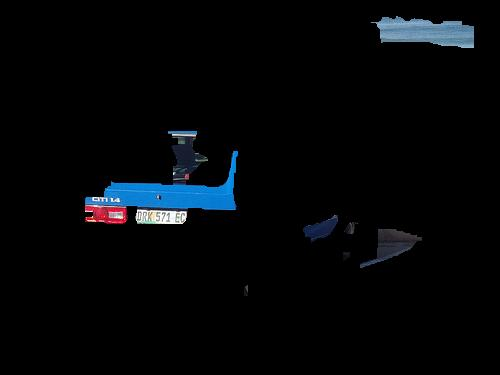
\includegraphics[width=2.95cm]{figures/sub_results/2008_007171_1_bad_sub.jpg.eps} &
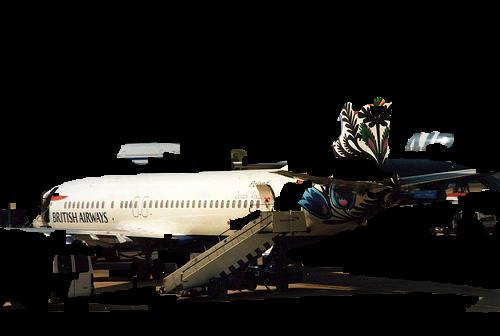
\includegraphics[width=2.95cm]{figures/sub_results/2008_000251_1_bad_sub.jpg.eps} \\
\end{tabular}
\caption{Selected results from segmentation of cars from the Pascal2008
dataset.  The first row shows the original image.  The second row shows
the best segmentation from the additive algorithm.  The third row shows
the segmentation from the subtractive algorithm with $f$ at different values
between 0.9 and 1.0.}
\label{fig:car_good_results}
\end{figure*}


\begin{figure*}[p]
\centering
\begin{tabular}{ p{3cm} p{3cm} p{3cm} p{3cm} }
\includegraphics[width=2.95cm]{figures/add_res/car/bad/2008_001961.jpg.eps} &
\includegraphics[width=2.95cm]{figures/add_res/car/bad/2008_003132.jpg.eps} &
\includegraphics[width=2.95cm]{figures/add_res/car/bad/2008_004312.jpg.eps} &
\includegraphics[width=2.95cm]{figures/add_res/car/bad/2008_004414.jpg.eps} \\

\includegraphics[width=2.95cm]{figures/add_res/car/bad/2008_001961.jpg_1_bad.jpg.eps} &
\includegraphics[width=2.95cm]{figures/add_res/car/bad/2008_003132.jpg_1_bad.jpg.eps} &
\includegraphics[width=2.95cm]{figures/add_res/car/bad/2008_004312.jpg_1_bad.jpg.eps} &
\includegraphics[width=2.95cm]{figures/add_res/car/bad/2008_004414.jpg_1_bad.jpg.eps} \\

\includegraphics[width=2.95cm]{figures/sub_results/good/2008_001961_0.80.jpg.eps} &
\includegraphics[width=2.95cm]{figures/sub_results/good/2008_003132_1.10.jpg.eps} &
\includegraphics[width=2.95cm]{figures/sub_results/good/2008_004312_1.00.jpg.eps} &
\includegraphics[width=2.95cm]{figures/sub_results/good/2008_004414_0.90.jpg.eps} \\

\end{tabular}
\caption{Selected results from segmentation of cars from the Pascal2008
dataset.  The first row shows the original image.  The second row shows
the best segmentation from the additive algorithm.  The third row shows
the segmentation from the subtractive algorithm with $f$ at different values
between 0.9 and 1.0.}
\label{fig:car_bad_results}
\end{figure*}



\begin{figure*}[p]
\centering
\begin{tabular}{ p{3cm} p{3cm} p{3cm} p{3cm} }
\includegraphics[width=2.95cm]{figures/add_res/plane/2008_000021.jpg.eps} &
\includegraphics[width=2.95cm]{figures/add_res/plane/2008_001971.jpg.eps} &
\includegraphics[width=2.95cm]{figures/add_res/plane/2008_002673.jpg.eps} &
\includegraphics[width=2.95cm]{figures/add_res/plane/2008_002138.jpg.eps} \\
\includegraphics[width=2.95cm]{figures/add_res/plane/2008_000021.jpg_2_good.jpg.eps} &
\includegraphics[width=2.95cm]{figures/add_res/plane/2008_001971.jpg_2_good.jpg.eps} &
\includegraphics[width=2.95cm]{figures/add_res/plane/2008_002673.jpg_2_good.jpg.eps} &
\includegraphics[width=2.95cm]{figures/add_res/plane/2008_002138.jpg_2_good.jpg.eps} \\
\end{tabular}
\caption{Selected results from segmentation of planes from the Pascal2008
dataset.  The first row shows the original image.  The second row shows
the best segmentation from the additive algorithm.}
\label{fig:aeroplane_good_results}
\end{figure*}


\begin{figure*}[p]
\centering
\begin{tabular}{ p{3cm} p{3cm} p{3cm} p{3cm} }
\includegraphics[width=2.95cm]{figures/add_res/plane/2008_000804.jpg.eps} &
\includegraphics[width=2.95cm]{figures/add_res/plane/2008_001805.jpg.eps} &
\includegraphics[width=2.95cm]{figures/add_res/plane/2008_002358.jpg.eps} &
\includegraphics[width=2.95cm]{figures/add_res/plane/2008_003673.jpg.eps} \\
\includegraphics[width=2.95cm]{figures/add_res/plane/2008_000804.jpg_2_bad.jpg.eps} &
\includegraphics[width=2.95cm]{figures/add_res/plane/2008_001805.jpg_2_okay.jpg.eps} &
\includegraphics[width=2.95cm]{figures/add_res/plane/2008_002358.jpg_2_okay.jpg.eps} &
\includegraphics[width=2.95cm]{figures/add_res/plane/2008_003673.jpg_2_bad.jpg.eps} \\
\end{tabular}
\caption{Selected results from segmentation of planes from the Pascal2008
dataset.  The first row shows the original image.  The second row shows
the best segmentation from the additive algorithm.}
\label{fig:aeroplane_bad_results}
\end{figure*}


\begin{figure*}[p]
\centering
\begin{tabular}{ p{3cm} p{3cm} p{3cm} p{3cm} }
\includegraphics[width=2.95cm]{figures/add_res/horse/2008_001542.jpg.eps} &
\includegraphics[width=2.95cm]{figures/add_res/horse/2008_001992.jpg.eps} &
\includegraphics[width=2.95cm]{figures/add_res/horse/2008_002172.jpg.eps} &
\includegraphics[width=2.95cm]{figures/add_res/horse/2008_002509.jpg.eps} \\
\includegraphics[width=2.95cm]{figures/add_res/horse/2008_001542.jpg_3_good.jpg.eps} &
\includegraphics[width=2.95cm]{figures/add_res/horse/2008_001992.jpg_3_good.jpg.eps} &
\includegraphics[width=2.95cm]{figures/add_res/horse/2008_002172.jpg_3_good.jpg.eps} &
\includegraphics[width=2.95cm]{figures/add_res/horse/2008_002509.jpg_3_good.jpg.eps} \\
\end{tabular}
\caption{Selected results from segmentation of horses from the Pascal2008
dataset.  The first row shows the original image.  The second row shows
the best segmentation from the additive algorithm.}
\label{fig:horse_good_results}
\end{figure*}


\begin{figure*}[p]
\centering
\begin{tabular}{ p{3cm} p{3cm} p{3cm} p{3cm} }
\includegraphics[width=2.95cm]{figures/add_res/horse/2008_000403.jpg.eps} &
\includegraphics[width=2.95cm]{figures/add_res/horse/2008_002835.jpg.eps} &
\includegraphics[width=2.95cm]{figures/add_res/horse/2008_003055.jpg.eps} &
\includegraphics[width=2.95cm]{figures/add_res/horse/2008_004470.jpg.eps} \\
\includegraphics[width=2.95cm]{figures/add_res/horse/2008_000403.jpg_3_bad.jpg.eps} &
\includegraphics[width=2.95cm]{figures/add_res/horse/2008_002835.jpg_3_bad.jpg.eps} &
\includegraphics[width=2.95cm]{figures/add_res/horse/2008_003055.jpg_3_okay.jpg.eps} &
\includegraphics[width=2.95cm]{figures/add_res/horse/2008_004470.jpg_3_bad.jpg.eps} \\
\end{tabular}
\caption{Selected results from segmentation of horses from the Pascal2008
dataset.  The first row shows the original image.  The second row shows
the best segmentation from the additive algorithm.}
\label{fig:horse_bad_results}
\end{figure*}


%-------------------------------------------------------------------------------
% conclusions and future work
%-------------------------------------------------------------------------------
\section{Discussion}
\label{sec:discussion}

It can be seen that in simple cases both additive and subtractive algorithms
are able to segment out rough outlines of the objects.  In most cases, even
the more difficult ones, at least part of the car was present in the final
segmentation.  This shows that the segmentation algorithms appear to be
reasonable approximations to a combinatoric approach -- that of predicting
on every combination of regions in the image.

Despite these encouraging initial results, the final segmentation region
was often not coherent.
This appears to be largely because the region tree approach is not
constrained by spatial coherence.  That is, two leaf nodes containing image
regions that are spatially next to each other may be very distant in the
region tree.  Because of this, the attribute distribution may change significantly
after considering the first node and before consideration of the second node.
Another reason for this may be that our canonical attribute distribution for
our objects gave equal weights to each attribute.  For example, a wheel was
equally as important as shininess.  This gave unfair disadvantages to
under-represented or ill-trained attributes.  This can be seen in the results
where the body of the car is removed while the wheels or headlights are
retained.

An interesting orthogonal direction that could be taken with these ideas is to
use segmentation using attributes as a diagnostic tool for attribute classifiers.
That is, the segmentations produced by our algorithms can help zero in on areas
in an image that exhibit high responses in detection of certain attributes.
For example, an image could be segmented using similarity to a canonical distribution
using only one attribute.  If that attribute is ``fur'' and segmentations
consistently show paws and tails, then it would quickly become clear that
the fur attribute classifier has learned on something other than fur.

As object classification is generally only as good as the features used, so also it
appears that this approach to segmentation is only as good as the attribute
selection and training.  We found that in images with poor segmentations, the
confidences in prediction of object-related attributes were generally low. Using bounding 
boxes as ground truth can introduce many background features into the attribute models. These 
features can be harmful. The extreme example is shown in the left image of figure \ref{fig:horse_bad_results}, 
which only segments out the background grass. However, even if we have the segmentation 
of objects as the ground truth for training the attributes, we may still not have accurate 
models, since the ground truth is for objects not for attributes. For example, if we train 
the attributes of wheel or metal only based on car images, we may get the car model not 
the attributes model. One way to deal with this problem is to directly label attributes 
ground truth. Then we can get similar accurate attribute models as the object models. 

Another problem with the attribute based method is that the attributes are not discriminative 
enough to separate different objects. For example, if we use the general attributes of head, torso and leg to 
do the object classification, we cannot separate dog and cat, since both of them have all of the attributes. 
But those attributes can definitely separate the two objects from non-animal objects, such as car. So
attributes are helpful for object classification, but they are often not discriminative enough. One way to deal with this is to use 
both attributes features and low level objects features for object classification. We can train general attributes models first. 
When we want to classify some specific objects, we can incorporate a small number of low level features from the specific object samples to the attributes 
features. In this way, we both reduce the training samples for object classification, and make the attribute based method more discriminative.

Interestingly, the region pruning algorithms are feature-type independent.  That
is, they are not necessarily wedded to attribute features and could be used with
any feature type given a similarity scoring function.  Interesting future work would
be to try the pruning methods with lower-level features.

The holy grail of this approach, of course, is to be able to segment any object
with a given canonical attribute distribution.  If this can be achieved, 
then segmentation experiments
could open up to non-experts, who could define an attribute distribution
based on their own knowledge and use a system that has already been trained
on a large number of attributes to segment the object.

\subsection*{Acknowledgements}
Thanks to the authors of \cite{arbelaez09} and \cite{farhadi09} for use of their
segmentation and feature extraction code, respectively.

%-------------------------------------------------------------------------------
% bibliography
%-------------------------------------------------------------------------------
{\small
%\bibliographystyle{plain}
\bibliographystyle{ieee}
\bibliography{refs}
}

\end{document}
